\IfFileExists{stacks-project.cls}{%
\documentclass{stacks-project}
}{%
\documentclass{amsart}
}

% For dealing with references we use the comment environment
\usepackage{verbatim}
\newenvironment{reference}{\comment}{\endcomment}
%\newenvironment{reference}{}{}
\newenvironment{slogan}{\comment}{\endcomment}
\newenvironment{history}{\comment}{\endcomment}

% For commutative diagrams we use Xy-pic
\usepackage[all]{xy}

% We use 2cell for 2-commutative diagrams.
\xyoption{2cell}
\UseAllTwocells

% We use multicol for the list of chapters between chapters
\usepackage{multicol}

% This is generally recommended for better output
\usepackage{lmodern}
\usepackage[T1]{fontenc}

% For cross-file-references
\usepackage{xr-hyper}

% Package for hypertext links:
\usepackage{hyperref}

% For any local file, say "hello.tex" you want to link to please
% use \externaldocument[hello-]{hello}
\externaldocument[introduction-]{introduction}
\externaldocument[conventions-]{conventions}
\externaldocument[sets-]{sets}
\externaldocument[categories-]{categories}
\externaldocument[topology-]{topology}
\externaldocument[sheaves-]{sheaves}
\externaldocument[sites-]{sites}
\externaldocument[stacks-]{stacks}
\externaldocument[fields-]{fields}
\externaldocument[algebra-]{algebra}
\externaldocument[brauer-]{brauer}
\externaldocument[homology-]{homology}
\externaldocument[derived-]{derived}
\externaldocument[simplicial-]{simplicial}
\externaldocument[more-algebra-]{more-algebra}
\externaldocument[smoothing-]{smoothing}
\externaldocument[modules-]{modules}
\externaldocument[sites-modules-]{sites-modules}
\externaldocument[injectives-]{injectives}
\externaldocument[cohomology-]{cohomology}
\externaldocument[sites-cohomology-]{sites-cohomology}
\externaldocument[dga-]{dga}
\externaldocument[dpa-]{dpa}
\externaldocument[sdga-]{sdga}
\externaldocument[hypercovering-]{hypercovering}
\externaldocument[schemes-]{schemes}
\externaldocument[constructions-]{constructions}
\externaldocument[properties-]{properties}
\externaldocument[morphisms-]{morphisms}
\externaldocument[coherent-]{coherent}
\externaldocument[divisors-]{divisors}
\externaldocument[limits-]{limits}
\externaldocument[varieties-]{varieties}
\externaldocument[topologies-]{topologies}
\externaldocument[descent-]{descent}
\externaldocument[perfect-]{perfect}
\externaldocument[more-morphisms-]{more-morphisms}
\externaldocument[flat-]{flat}
\externaldocument[groupoids-]{groupoids}
\externaldocument[more-groupoids-]{more-groupoids}
\externaldocument[etale-]{etale}
\externaldocument[chow-]{chow}
\externaldocument[intersection-]{intersection}
\externaldocument[pic-]{pic}
\externaldocument[weil-]{weil}
\externaldocument[adequate-]{adequate}
\externaldocument[dualizing-]{dualizing}
\externaldocument[duality-]{duality}
\externaldocument[discriminant-]{discriminant}
\externaldocument[derham-]{derham}
\externaldocument[local-cohomology-]{local-cohomology}
\externaldocument[algebraization-]{algebraization}
\externaldocument[curves-]{curves}
\externaldocument[resolve-]{resolve}
\externaldocument[models-]{models}
\externaldocument[functors-]{functors}
\externaldocument[equiv-]{equiv}
\externaldocument[pione-]{pione}
\externaldocument[etale-cohomology-]{etale-cohomology}
\externaldocument[proetale-]{proetale}
\externaldocument[relative-cycles-]{relative-cycles}
\externaldocument[more-etale-]{more-etale}
\externaldocument[trace-]{trace}
\externaldocument[crystalline-]{crystalline}
\externaldocument[spaces-]{spaces}
\externaldocument[spaces-properties-]{spaces-properties}
\externaldocument[spaces-morphisms-]{spaces-morphisms}
\externaldocument[decent-spaces-]{decent-spaces}
\externaldocument[spaces-cohomology-]{spaces-cohomology}
\externaldocument[spaces-limits-]{spaces-limits}
\externaldocument[spaces-divisors-]{spaces-divisors}
\externaldocument[spaces-over-fields-]{spaces-over-fields}
\externaldocument[spaces-topologies-]{spaces-topologies}
\externaldocument[spaces-descent-]{spaces-descent}
\externaldocument[spaces-perfect-]{spaces-perfect}
\externaldocument[spaces-more-morphisms-]{spaces-more-morphisms}
\externaldocument[spaces-flat-]{spaces-flat}
\externaldocument[spaces-groupoids-]{spaces-groupoids}
\externaldocument[spaces-more-groupoids-]{spaces-more-groupoids}
\externaldocument[bootstrap-]{bootstrap}
\externaldocument[spaces-pushouts-]{spaces-pushouts}
\externaldocument[spaces-chow-]{spaces-chow}
\externaldocument[groupoids-quotients-]{groupoids-quotients}
\externaldocument[spaces-more-cohomology-]{spaces-more-cohomology}
\externaldocument[spaces-simplicial-]{spaces-simplicial}
\externaldocument[spaces-duality-]{spaces-duality}
\externaldocument[formal-spaces-]{formal-spaces}
\externaldocument[restricted-]{restricted}
\externaldocument[spaces-resolve-]{spaces-resolve}
\externaldocument[formal-defos-]{formal-defos}
\externaldocument[defos-]{defos}
\externaldocument[cotangent-]{cotangent}
\externaldocument[examples-defos-]{examples-defos}
\externaldocument[algebraic-]{algebraic}
\externaldocument[examples-stacks-]{examples-stacks}
\externaldocument[stacks-sheaves-]{stacks-sheaves}
\externaldocument[criteria-]{criteria}
\externaldocument[artin-]{artin}
\externaldocument[quot-]{quot}
\externaldocument[stacks-properties-]{stacks-properties}
\externaldocument[stacks-morphisms-]{stacks-morphisms}
\externaldocument[stacks-limits-]{stacks-limits}
\externaldocument[stacks-cohomology-]{stacks-cohomology}
\externaldocument[stacks-perfect-]{stacks-perfect}
\externaldocument[stacks-introduction-]{stacks-introduction}
\externaldocument[stacks-more-morphisms-]{stacks-more-morphisms}
\externaldocument[stacks-geometry-]{stacks-geometry}
\externaldocument[moduli-]{moduli}
\externaldocument[moduli-curves-]{moduli-curves}
\externaldocument[examples-]{examples}
\externaldocument[exercises-]{exercises}
\externaldocument[guide-]{guide}
\externaldocument[desirables-]{desirables}
\externaldocument[coding-]{coding}
\externaldocument[obsolete-]{obsolete}
\externaldocument[fdl-]{fdl}
\externaldocument[index-]{index}

% Theorem environments.
%
\theoremstyle{plain}
\newtheorem{theorem}[subsection]{Theorem}
\newtheorem{proposition}[subsection]{Proposition}
\newtheorem{lemma}[subsection]{Lemma}

\theoremstyle{definition}
\newtheorem{definition}[subsection]{Definition}
\newtheorem{example}[subsection]{Example}
\newtheorem{exercise}[subsection]{Exercise}
\newtheorem{situation}[subsection]{Situation}

\theoremstyle{remark}
\newtheorem{remark}[subsection]{Remark}
\newtheorem{remarks}[subsection]{Remarks}

\numberwithin{equation}{subsection}

% Macros
%
\def\lim{\mathop{\mathrm{lim}}\nolimits}
\def\colim{\mathop{\mathrm{colim}}\nolimits}
\def\Spec{\mathop{\mathrm{Spec}}}
\def\Hom{\mathop{\mathrm{Hom}}\nolimits}
\def\Ext{\mathop{\mathrm{Ext}}\nolimits}
\def\SheafHom{\mathop{\mathcal{H}\!\mathit{om}}\nolimits}
\def\SheafExt{\mathop{\mathcal{E}\!\mathit{xt}}\nolimits}
\def\Sch{\mathit{Sch}}
\def\Mor{\mathop{\mathrm{Mor}}\nolimits}
\def\Ob{\mathop{\mathrm{Ob}}\nolimits}
\def\Sh{\mathop{\mathit{Sh}}\nolimits}
\def\NL{\mathop{N\!L}\nolimits}
\def\CH{\mathop{\mathrm{CH}}\nolimits}
\def\proetale{{pro\text{-}\acute{e}tale}}
\def\etale{{\acute{e}tale}}
\def\QCoh{\mathit{QCoh}}
\def\Ker{\mathop{\mathrm{Ker}}}
\def\Im{\mathop{\mathrm{Im}}}
\def\Coker{\mathop{\mathrm{Coker}}}
\def\Coim{\mathop{\mathrm{Coim}}}

% Boxtimes
%
\DeclareMathSymbol{\boxtimes}{\mathbin}{AMSa}{"02}

%
% Macros for moduli stacks/spaces
%
\def\QCohstack{\mathcal{QC}\!\mathit{oh}}
\def\Cohstack{\mathcal{C}\!\mathit{oh}}
\def\Spacesstack{\mathcal{S}\!\mathit{paces}}
\def\Quotfunctor{\mathrm{Quot}}
\def\Hilbfunctor{\mathrm{Hilb}}
\def\Curvesstack{\mathcal{C}\!\mathit{urves}}
\def\Polarizedstack{\mathcal{P}\!\mathit{olarized}}
\def\Complexesstack{\mathcal{C}\!\mathit{omplexes}}
% \Pic is the operator that assigns to X its picard group, usage \Pic(X)
% \Picardstack_{X/B} denotes the Picard stack of X over B
% \Picardfunctor_{X/B} denotes the Picard functor of X over B
\def\Pic{\mathop{\mathrm{Pic}}\nolimits}
\def\Picardstack{\mathcal{P}\!\mathit{ic}}
\def\Picardfunctor{\mathrm{Pic}}
\def\Deformationcategory{\mathcal{D}\!\mathit{ef}}

%Dani's additions
\usepackage{graphicx} %figures


\begin{document}

\title{Differential Geometry}
\maketitle

\phantomsection
\label{section-phantom}
\hfill
\href{http://github.com/danimalabares/stack}{github.com/danimalabares/stack}
\tableofcontents

\section{Differential of a map}
\label{section-differential}

\section{Riemannian metrics}
\label{section-Riemannian-metrics}

\begin{definition}
\label{definition-product-metric}
Let $M_1$ and $M_2$ be Riemannian manifolds. The {\it product metric} on
$M_1\times M_2$ is $\pi_1^*g_1+\pi_2^*g_2$.
\end{definition}

\begin{definition}
\label{definition-flat-torus}
$S^1\times\ldots\times S^1$ with the product metric is called the {\it flat
torus}.
\end{definition}

\begin{exercise}[Warped product]
\label{exercise-wraped-product}
See \cite{pet}. Para $(M,g_M)$ e $(N,g_N)$ e $f:M \to \mathbb{R}_+$, definimos o
 {\it warped product} como sendo o produto cartesiano $M\times N$ com a métrica 
 $g_M+f^2g_N$.

Mostre que se os fatores são completos, o warped product é completo.
\end{exercise}

\begin{definition}
\label{definition-gradient}
Let  $f:M\to\mathbb{R}$. Define the {\it gradient} of $f$ as the (unique) vector
field $\nabla f$ such that
\begin{equation}
\label{equation-gradient}
\left<\nabla f,X\right>=Xf, \qquad \forall X\in\mathfrak{X}(M).
\end{equation}
\end{definition}

Notice that for a frame $E_i$ with dual frame $E^i$ we have
\begin{align*}
\left<\nabla f,X\right>&=g_{ij}E^i\odot E^j(\nabla f,X)
=g_{ij}(\nabla f)^iX^j\\
Xf&=df(X)=(df)_iE^i(X)=(df)_iX^i\\
\implies& g^{ij}(df)_iX^j=(\nabla f)^iX^i
\end{align*}
so substituting $X$ with a basic vector $E_i$ and $(df)_i$ with $\partial_if$ we
obtain
\begin{equation}
\label{equation-gradient-in-coordinates}
(\nabla f)^i=g^{ij}\partial_if \iff \nabla f=g^{ij}\partial_ifE_j
\end{equation}

\begin{definition}
\label{definition-divergence}
For any $X\in \mathfrak{X}(M)$,
$$
\text{div}(X):=\text{tr}(v\mapsto \nabla_vX)
$$
\end{definition}

\begin{lemma}
\label{lemma-Laplacian-of-product}
\cite{doc}, Chapter III, Exercise 9(b).
\begin{equation}
\label{equation-Laplacian-of-product}
\Delta(fg)=f \Delta g + g \Delta f+2\left<\nabla f,\nabla g\right>
\end{equation}
\end{lemma}

\begin{proof}
Just compute.
\end{proof}

\begin{lemma}
\label{lemma-divergence-and-volume}
\begin{equation}
\label{equation-divergence-and-volume}
di_X\text{Vol}=\text{div}X\text{Vol},\qquad \text{for all }X\in \mathfrak{X}(M).
\end{equation}
\end{lemma}

\begin{proof}
Pick a geodesic frame $E_i$ (see Lemma \ref{lemma-geodesic-coordinates}) and
its dual coframe $\varepsilon^i$, i.e. satisfying
$\varepsilon^i(E_j)=\delta_{ij}$. Then $\operatorname{Vol}=\varepsilon^1
\wedge \ldots \wedge \varepsilon^n$. Then for any $X=X^iE_i \in
\mathfrak{X}(U)$,

\begin{align*}
i_X\operatorname{Vol}
&=\varepsilon^1\wedge\ldots\wedge\varepsilon^n(X^iE_i,\cdot,\ldots,\cdot)
=X^i\varepsilon^1\wedge\ldots\wedge\varepsilon^n(E_i,\cdot,\ldots,\cdot)
\end{align*}
How to compute that? Recall that for top-forms we have
$$
\varepsilon^1\wedge\ldots\wedge\varepsilon^n(Z_1,\ldots,Z_n)
=\det(\varepsilon^i(Z_j))
$$
so for example if $n=3$
\begin{align*}\varepsilon^1\wedge \varepsilon^2\wedge\varepsilon^3(E_1,Z_2,Z_3)
&=\begin{vmatrix}
\varepsilon^1(E_1)&\varepsilon^1(Z_2) &\varepsilon^1(Z_3)\\
\varepsilon^2(E_1)&\varepsilon^2(Z_2)&\varepsilon^2(Z_3)\\
\varepsilon^3(E_1)&\varepsilon^3(Z_2)&\varepsilon^3(Z_3)
\end{vmatrix}
=\begin{vmatrix}
1&\varepsilon^1(Z_2) &\varepsilon^1(Z_3)\\
0&\varepsilon^2(Z_2)&\varepsilon^2(Z_3)\\
0&\varepsilon^3(Z_2)&\varepsilon^3(Z_3)
\end{vmatrix}\\
&=\varepsilon^2(Z_2)\varepsilon^3(Z_3)-\varepsilon^2(Z_3)\varepsilon^3(Z_2)
=\varepsilon^2\wedge\varepsilon^3(Z_2,Z_3),\\
\varepsilon^1\wedge\varepsilon^2\wedge\varepsilon^3(E_2,Z_2,Z_3)
&=\begin{vmatrix}
0&\varepsilon^1(Z_2) &\varepsilon^1(Z_3)\\
1&\varepsilon^2(Z_2)&\varepsilon^2(Z_3)\\
0&\varepsilon^3(Z_2)&\varepsilon^3(Z_3)
\end{vmatrix}=-\varepsilon^1\wedge\varepsilon^3(Z_2,Z_3)
\end{align*}
and so on. When we sum over all $i$, we get
$$
X^i\varepsilon^1\wedge\ldots\wedge\varepsilon^n(E_i,\cdot,\ldots,\cdot)
=\sum_{i}(-1)^{i+1}X^i\varepsilon^1\wedge\ldots\wedge\widehat{\varepsilon^i}
\wedge\ldots\wedge\varepsilon^n.
$$
Now take exterior derivative of that, we get
\begin{align*}
d i_X\operatorname{Vol}
&=\sum_i(-1)^{i+1}(dX^i)\wedge\varepsilon^1\wedge\ldots
\wedge\widehat{\varepsilon^i}\wedge\ldots\wedge\varepsilon^n\\
&+\sum_{i}(-1)^{i+1}X^i\wedge 
d(\varepsilon^1\wedge\ldots\wedge\widehat{\varepsilon^i}\wedge\ldots
\wedge\varepsilon^n)\end{align*}
And then the first term actually is
\begin{align*}
\sum_i(-1)^{i+1}E_jX^i\varepsilon^j\wedge\varepsilon^1\wedge\ldots
\wedge\widehat{\varepsilon^i}\wedge\ldots\wedge\varepsilon^n
&=E_iX^i\operatorname{Vol}
\end{align*}
while the second term vanishes because look,
\begin{align*}d \varepsilon^i(E_j,E_k)
&=E_j\varepsilon^i(E_k)-E_k\varepsilon^i(E_j)-\varepsilon^i([E_j,E_k])\\
&=-\varepsilon^i(\nabla_{E_j}E_k-\nabla_{E_k}E_j)\qquad \text{torsion!}
\end{align*}
which vanishes at $p$ because we said that this geodesic frame would have
 vanishing Christoffel symbols at $p$. So we conclude:
\[di_X \operatorname{Vol}=E_iX^i\operatorname{Vol}\]

Now you just have to think what is divergence:
\begin{align*}
\operatorname{div}X&=\sum_{i}\left<\nabla_{E_i}X^jE_j,E_i\right>
=\sum_{i}\left<E_iX^jE_j,E_i\right>+X^j\left<\nabla_{E_i}E_j,E_i\right>\\
&=\sum_i \left<E_iX^jE_j,E_i\right>=\sum_iE_iX^j\left<E_j,E_i\right>=E_iX^i
\end{align*}
again using that we are a geodesic frame with vanishing covariant 
derivative at $p$.
\end{proof}

\section{Connections}
\label{section-connections}

\begin{example}
\label{example-euclidean-connection}
The usual connection in $\mathbb{R}^n$ is given by 
$$
\nabla_XY=X(Y^i)\partial_i
$$
\end{example}

\begin{proposition}[Everything I know about connections]
\label{proposition-existence-of-pullback-connection}
\end{proposition}

\begin{lemma}
\label{lemma-composition-of-pullback-connections}
\cite{aulas}, p.5. If $g:M_1\to M_2$ and $f:M_2\to M_3$ are smooth maps of 
manifolds and $E$ is a vector bundle over $M_3$, then
$$
g^* (f^* (E))=(f\circ g)^* (E)\qquad \text{and}\qquad
(\nabla^f)^g=\nabla^{f\circ g}
$$
\end{lemma}

The following three lemmas are fundamental properties of isometric
immersions and will be used in Section \ref{section-isometric-immersions}. (Cf.
Lista 3, Exercise 2.)

\begin{lemma}
\label{lemma-tangent-component-of-pullback-connection-by-ii-is-LC}
If $f:M \to \tilde{M}$ is an isometric immersion, then 
$f_*(\nabla_XY)=(\nabla^f_Xf_*Y)^\top$.
\end{lemma}

\begin{proof}
We have to check that $(\nabla^f_Xf_*Y)^\top$ is a torsion-free and compatible
connection on $TM$.
\end{proof}

\begin{lemma}
\label{lemma-isometric-immersion-along-curve}
Let $f:M \to \tilde{M}$ be an isometric immersion, $c$ is a smooth curve in $M$
and $Y\in\mathfrak{X}_c$. Then
$$
f_*\nabla_{\frac{d}{dt}}^\gamma Y
=\left(\nabla^{f\circ\gamma}_{\frac{d}{dt}}f_*Y\right)^\top
$$
\end{lemma}

\begin{proof}
This is just a mixture of Lemmas \ref{lemma-composition-of-pullback-connections}
 and \ref{lemma-tangent-component-of-pullback-connection-by-ii-is-LC}.
\end{proof}

The following result will be reminded when we define totally geodesic
submanifolds, cf. Definition \ref{definition-totally-geodesic-submanifold},
addressing the case when also the normal component vanishes:

\begin{lemma}
\label{lemma-geodesics-of-submanifold-characterization}
Let $f:M \to \tilde{M}$ be an isometric immersion and $\gamma:I\to M$ a smooth
curve parametrized by arclength. Show that $\gamma$ is a geodesic of M
if and only if its acceleration on $\tilde{M}$ is perpendicular to $M$, that is,
$$
\tilde{\nabla}^{f\circ\cong\gamma}_{\frac{d}{dt}}(f\circ\gamma)'\perp
f_*(T_{\gamma(t)}M)
$$
\end{lemma}

\begin{proof}
Decompose the vector field 
$\tilde{\nabla}^{f\circ\cong\gamma}_{\frac{d}{dt}}(f\circ\gamma)'$ in tangent and
normal part. Then apply Lemma 
\ref{lemma-tangent-component-of-pullback-connection-by-ii-is-LC}.
\end{proof}

\section{Riemannian submersions and immersions}
\label{section-Riemannian-submersions-and-immersions}

For any smooth manifold submersion $\pi:\tilde{M}\to M$ there is a bundle
isomorphism I love: 
\begin{equation}
\label{equation-submersion-bundle-decomposition}
\pi^*TM \oplus \Ker \pi\cong
T\tilde{M} \end{equation}
 where $\Ker\pi$ is the {\it kernel bundle}, whose
fiber is the kernel of $\pi_*$, and is also called the {\it vertical bundle}.
Proving that $\Ker\pi$ is in fact a bundle and confirming the isomorphism
\ref{equation-submersion-bundle-decomposition} is a simple exercise.

We call $\pi$ a {\it riemannian submersion} only when $\pi^*TM$ is isometric to
$TM$, which makes sense only when $\tilde{M}$ and $M$ are Riemannian manifolds.

Following notation of \cite{Milnor-Characteristic-Classes}, for any subbundle
$\xi \subset\eta$ over a Riemannian manifold, the {\it orthogonal complement
bundle} $\xi^\perp$ can be defined fiberwise as the orthogonal complement of the
fiber and shown to be a bundle as in the case of the kernel bundle. Then Milnor
defines the {\it normal bundle} when $\xi$ is the tangent bundle of a
submanifold. Finally this construction is noted to work just as well for any
isometric immersion $f:M\to \tilde{M}$, so that
\begin{equation}
\label{equation-immersion-bundle-decomposition}
f^*T\tilde{M}\cong TM\oplus T^\perp M
\end{equation}
Further, in problem 3-B we are asked to define for $\xi \subset \eta$ the {\it
quotient bundle} and show it's a bundle. And if $\eta$ has a Riemannian metric,
then $\xi^\perp\cong\eta/\xi$. So that's why we sometimes say that we can define
the normal bundle using a Riemannian metric but we don't need to.

An interesting thought is: given a subbundle, is there a manifold whose tangent
bundle is that subbundle?

\section{Geodesics}
\label{section-geodesics}

\begin{example}[Geodesics of sphere]
\label{example-geodesics-of-Sn}
The geodesics of $S^n$ are 
\begin{equation}
\label{equation-geodesics-of-Sn}
\gamma(t)=\cos t p+\sin t v
\end{equation}
for $p \in S^n$ and $v\in T^1_pS^n$.

Derivando como uma simples curva em $\mathbb{R}^{n+1}$, vemos que
$\gamma''=-\gamma$, o que significa que $(\gamma'')^{\top}=0$, i.e. $\gamma$ é
uma geodésica de $\mathbb{S}^n$.

Sendo essa uma geodésica partindo de um ponto arbitrário numa direção
arbitrária, concluimos por unicidade das geodésicas e \textit{rescaling lemma}
que todas as geodésicas de $\mathbb{S}^n$ são como $\gamma$.
\end{example}

\begin{example}[Isometry group of sphere]
\label{example-isometry-group-of-Sn}
The isometry group of $S^n$ is
$$
\text{O}(n):=\{A\in\text{GL}(n+1):AA^{\mathbf{T}}=\text{Id}\}
$$
It's immediate that $\mathcal{O}(n+1)\subset \text{Isom}(S^n)$ since orthogonal
transformations preserve euclidean product:
\begin{align*}
A A^{\mathbf{T}}&=\text{Id}\iff \sum_k A_{ik}A_{jk}=\delta_{ij}
\iff Ae_i\cdot Ae_j=\delta_{ij}\\ 
\iff Av\cdot Aw&= A\left( v^ie_i\right) \cdot A\left( w^je_j\right) 
=v^iw^j (Ae_i)\cdot (Ae_j)
=v^i\cdot w^j\delta_{ij}=v\cdot w
\end{align*}
For the other contention let $A:S^n \to S^n$ be an isometry.

Vamos mostrar que $A$ é a restrição de uma função $\tilde{A} \in
\mathsf{O}(n+1)$. Defina
\begin{align*}
\tilde{A}: \mathbb{R}^{n+1} &\longrightarrow \mathbb{R}^{n+1} \\
(r,\theta) &\longmapsto rA(1,\theta)\\
0&\longmapsto 0
\end{align*}
Se mostramos que $\tilde{A}$ é uma isometria linear, é claro que ela é um
elemento de $\mathsf{O}(n+1)$ pela conta anterior. De fato, basta mostrar que
$\tilde{A}$ é uma isometria, pois toda isometria de espaços de Banach que fixa
a origem é linear (\cite{braga} Teo. 7.11).

Para ver que $\tilde{A}$ é uma isometria de $\mathbb{R}^{n+1}$,
afirmo que a distância de $p$ a $q$ está totalmente determinada
pelas normas  $\|p\|$ e $\|q\|$, e pela distancia esférica entre
$\frac{p}{\|p\|}$ e $\frac{q}{\|q\|}$. Note que essa afirmação é na verdade
um problema de geometria plana, pois todas essas quantidades podem ser descritas
dentro do único plano que contém $0$, $p$ e $q$.

Acabou que essa afirmação é simplesmente a lei dos cosenos, já que a distância
esférica entre $\frac{p}{\|p\|}$ e $\frac{q}{\|q\|}$ é exatamente o angulo
entre $p$ e $q$ (poque essa distância é um segmento de círculo máximo!):
\[\text{lei dos cosenos:} \qquad d(p,q)^2=\|p\|^2+\|q\|^2-2\|p\|\|q\| \cos
\angle(p,q) \]

Em fim, $\tilde{A}$ é uma isometria porque
$d_{\mathbb{R}^{n+1}}(p,q)=d_{\mathbb{R}^{n+1}}(\tilde{A}p,\tilde{A}q)$ pelo
argumento anterior.
\end{example}

\begin{proposition}
\label{proposition-naturallity-of-exponential}
If $f:M\to \tilde{M}$ is an isometry,
$$
\xymatrix{
B_\varepsilon(0)\subset T_pM \ar[r]^{d_p f} \ar[d]_{\text{exp}_p} &
B_\varepsilon(0)\subset T_{f(p)}\tilde{M} \ar[d]^{\text{exp}_{f(p)}} \\
B_\varepsilon(p)\subset M \ar[r]_{f} & B_\varepsilon(f(p))\subset \tilde{M}
}
$$
\end{proposition}

\begin{proof}
Isometry maps geodesics to geodesics by Lemma 
\ref{lemma-isometry-maps-geodesics-to-geodesics}, then uniqueness of solutions
of ODEs.
\end{proof}

\begin{proposition}[Totally Normal Neighbourhoods]
\label{proposition-totally-normal-neighbourhoods}
For all $p \in M$ there is a neighbourhood $W \ni p$ and a number $\delta>0$ 
 such that for every $q \in W$, $B_\delta(q)$ is normal and
 $W \subset B_\delta(q)$. 
\end{proposition}

\begin{lemma}
\label{lemma-geodesic-coordinates}
At every point $p$ in $M$ there is an orthonormal frame 
$\{E_i\} \subset \mathfrak{X}(U)$ such that 
\begin{equation}
\label{equation-normal-coordinates-vanishing-Christoffel-symbols}
\Big(\nabla_{E_i}E_j\Big)_p=0
\end{equation}
(This means the Christoffel symbols of the connection vanish at the point $p$.)
\end{lemma}

\begin{proof}
This frame can be obtained by taking geodesic coordinates at the point, an
orthonormal base $\{e_i\}$ of $T_pM$, and taking parallel transport of the
vectors $e_i$ along radial geodesics emanating from $p$. This immediately
ensures that $E_i$ is orthonormal since parallel transport preserves angles.

To check that Christoffel symbols vanish at $p$ we do as follows. 
Take a random vector $v \in T_pM$ and its geodesic
$\gamma_v(t)=\operatorname{exp}_p(tv)$. I drop the subindex $v$ for the next
computations for the next computations. Then
\begin{align*}
0&=\nabla_{\frac{d}{dt}}^{\gamma}\gamma'
=\nabla^{\gamma}_{\frac{d}{dt}}v^i(E_i\circ \gamma)
\end{align*}
where the $v=(v^1,\ldots,v^n)$. Indeed: this is very silly but, since the 
coordinate chart of geodesic coordinates is $\operatorname{exp}_p^{-1}$, 
the coordinate representation of $\gamma$ in this chart is as simple as
$$
\hat{\gamma}(t)=(\underbrace{\varphi}_{\text{chart}} \circ \gamma)(t)
=\operatorname{exp}_p^{-1} \operatorname{exp}_p(tv)=tv.
$$
And the composition $E_i \circ \gamma$ just means that we take our local 
frame \textit{along $\gamma$}. Continue:
\begin{align*}
&=v^i\nabla^{\gamma}_{\frac{d}{dt}}E_i\circ\gamma
=v^i\nabla_{\gamma_{v,*} \frac{d}{dt}}E_i\\
&=v^i\nabla_{v^jE_j}E_i=v^iv^j\nabla_{E_j}E_i\\&
=v^iv^j\Gamma_{ji}^kE_k
\end{align*}
along $\gamma$. Now choose $v=e_1$. You get $\Gamma_{11}^k=0$ for all $k$ along $\gamma_{e_1}$. Now choose $v=e_2$, then $\Gamma_{22}^k=0$ along $\gamma_{e_2}$, so at least at $p$ they both vanish. And now choose $v=e_1+e_2$. You get
\begin{align*}
0=(v^1)^2 \underbrace{\Gamma_{1 1}^k}_{=0}
+v^1v^2 \Gamma_{1 2}^k+v^2v^1\Gamma_{2 1}^k
+(v^2)^2\underbrace{\Gamma_{2 2}^k}_{=0}
\end{align*}
So $\Gamma_{12}^k=0$ since Levi-Civita is torsion-free, i.e. symmetric. 
And so on. So the all Christoffel symbols vanish at the same time at $p$.
\end{proof}

\begin{exercise}
\label{exercise-maximum-principle}
\cite{doc}, Chapter III, Exercise 12. If $f$ is {\it subharmonic}, i.e. 
$\Delta f\geq 0$, on $M$ 
compact connected $\implies$ $f$ constant.
\end{exercise}

\begin{proof}
To prove the theorem for subharmonic functions first we show that in fact they
are harmonic via Eq. \ref{equation-divergence-and-volume} 
on $X:= \nabla f$ and Stokes:
$$
\int_M \Delta f \operatorname{Vol}=\int_M \operatorname{div}X \operatorname{Vol}
=\int_M d(i_X \operatorname{Vol})=\int_{\partial M}i_X \operatorname{Vol}=0
$$
meaning that the non-negative function $\Delta f$ is in fact 0, i.e. $f$ is
harmonic. Now we do it again for $X:=\nabla(f^2/2)$:
$$
\int_M \Delta(f^2/2)\operatorname{Vol}
=\int_M d(i_X \operatorname{Vol})
=\int_{\partial M}i_X \operatorname{Vol}
=0
$$
And then apply Eq. \ref{equation-Laplacian-of-product}:
$$
0=\int_M \Delta(f^2/2)\operatorname{Vol}
=\int_M f \Delta f \operatorname{Vol}
+\int_M \left<\nabla f,\nabla f\right>\operatorname{Vol}
$$
First one vanishes because $f$ is harmonic, so second one is zero which says
 $f$ is constant!
\end{proof}

\section{Curvature}
\label{section-curvature}

The {\it curvature tensor} is
\begin{equation}
\label{equation-curvature-tensor}
R(X,Y)Z=\nabla_X\nabla_YZ-\nabla_Y\nabla_XZ-\nabla_{[X,Y]}Z
\end{equation}

\begin{proposition}
\label{proposition-symmetries-of-curvature-tensor}
The curvature tensor is a tensor and
\begin{enumerate}
\item It is antisymmetric in the first two and last two entries,
\item $\left<R(X,Y)Z,W\right>=\left<R(Z,W)X,Y\right>$, and
\item Bianchi identity.
\end{enumerate}
\end{proposition}

Given a dimension-2 vector subspace $\sigma\subset T_pM$, the {\it sectional
curvature} of $M$ in $\sigma$ is
\begin{equation}
\label{equation-sectional-curvature}
K(\sigma)=\frac{\left<R(u,v)v,u\right>}
{\left<u,u\right>\left<v,v\right>-\left<u,v\right>^2}
\end{equation}
for any base $\{u,v\}$ of $\sigma$.

\begin{lemma}
\label{lemma-sectional-curvature-is-well-defined}
Sectional curvature does not depend on the choice of base.
\end{lemma}

\begin{proposition}
\label{proposition-curvature-like-tensor-determined-by-sectional-curvature}
Let $R$ and $R'$ be two type $(0,4)$ tensors on a vector space $\mathbb{V}$. If
their associated sectional curvatures $K$ and $K'$ are equal, then so are $R$
and $R'$.
\end{proposition}

\begin{proof}
Polarize and make lots of computations, cf. \cite{doc}.
\end{proof}

If a manifold has constant sectional curvature $c$,
\begin{equation}
\label{equation-constant-curvature}
\left<R(X,Y)Z,W\right>=
c(\left<X,Z\right>\left<Y,W\right>-\left<X,W\right>\left<Z,Y\right>)
\end{equation}
since the right-hand-side of Eq. \ref{equation-constant-curvature} is a
so-called curvature tensor, i.e. a tensor satisfying the symmetries of $R$, and
applying Proposition 
\ref{proposition-curvature-like-tensor-determined-by-sectional-curvature}.

The {\it Ricci tensor} is
\begin{equation}
\label{equation-Ricci-tensor}
\begin{aligned}
\text{Ric}: TM\times TM &\longrightarrow \mathbb{R} \\
\text{Ric}(X,Y)&=\frac{1}{n-1}\text{tr}(Z\mapsto R(Z,X)Y)
\end{aligned}
\end{equation}
It is symmetric.

The {\it Ricci curvature} is
\begin{equation}
\label{equation-Ricci-curvature}
\begin{aligned}
\text{Ric}: T^1M &\longrightarrow \mathbb{R} \\
\text{Ric}(X)=\text{Ric}(X,X)&=\frac{1}{n-1}\sum_{i=1}^{n-1}K(X,E_i)
\end{aligned}
\end{equation}
where $\{X,E_1,\ldots,E_{n-1}\}$ is an orthonormal basis.

The {\it scalar curvature} is
\begin{equation}
\label{equation-scalar-curvature}
\begin{aligned}
\text{scal}: M &\longrightarrow \mathbb{R} \\
\text{scal}(p)&=\frac{1}{n}\text{tr}\text{Ric}
=\frac{1}{n}\sum_i\text{Ric}(E_i,E_i)
\end{aligned}
\end{equation}

\begin{lemma}
\label{lemma-scalar-curvature-is-mean-of-sectional}
$$
\text{scal}(p)=\frac{1}{n}\sum_{i}\text{Ric}(e_i,e_i)
=\frac{1}{n(n-1)}\sum_{i,j}K(e_i,e_j)
=\frac{1}{\text{Vol}(S^{n-1})}\int_{\sigma\subset T_pM}K(\sigma)
$$
\end{lemma}

\begin{exercise}
\label{lemma-curvatures-of-product-metric}
Lista 5, Exercise 1. Let $(M_1,g_1)$ and $(M_2,g_2)$ be Riemannian manifolds and
let $M_1\times M_2$ be equipped with the product metric $g:=g_1\oplus g_2$. Show
that the curvature tensor, the Ricci curvature and the scalar curvature of $g$
are given by
\begin{enumerate}
\item $R=\pi_1^*R_1+\pi_2^*R^2$,
\item $\text{Ric}=\pi_1^*\text{Ric}_1+\pi_2^*\text{Ric}_2$,
\item $\text{scal}=\pi_1^*\text{scal}_1+\pi_2^*\text{scal}_2$
\end{enumerate}
where $\pi_i:M_1\times M_2\to M_i$ are the projections.
\end{exercise}

\begin{example}[Curvature of complex projective space]
\label{example-curvature-of-CPn}
Defina uma métrica Riemanniana  em $\mathbb{C}^{n+1}\setminus\{0\}$ do
seguinte modo. Se $Z \in \mathbb{C}^{n+1}\setminus\{0\}$ e $V,W \in T_Z
(\mathbb{C}^{n+1}\setminus\{0\})$,

$$
\left<V,W\right>_Z=\frac{\text{Re}(V,W)}{(Z,Z)}
$$
onde 
$$
(Z,W)=z_0\overline{w}_0+\ldots+z_n\overline{w}_n
$$

é o produto hermitiano em $\mathbb{C}^{n+1}$. Observe que a métrica
$\left<\cdot,\cdot\right>$ restrita a $S^{2n+1}\subset
\mathbb{C}^{n+1}\setminus\{0\}$ coincide com a métrica induzida por
$\mathbb{R}^{2n+2}$.
\begin{enumerate}

\item Mostre que, para todo $0\leq \theta \leq 2\pi$, $e^{i\theta}:S^{2n+1}\to
S^{2n+1}$ é uma isometria, e que, portanto, é possível definir uma métrica
Riemanniana em $\mathbb{P}^n(\mathbb{C})$ de modo que a submersão $f$ seja
Riemanniana.

\item Mostre que, nesta métrica, a curvatura seccional de
$\mathbb{P}^n(\mathbb{C})$ é dada por
$$
K(\sigma)=1+3\cos^2\varphi
$$
onde $\sigma$ é gerado pelo par ortonormal $X$, $Y$, $\cos
\varphi=\left<\overline{X},i\overline{Y}\right>$, e $\overline{X}$,
$\overline{Y}$ são os levantamentos horizontais de $X$ e $Y$, respetivamente. Em
particular, $1 \leq  K(\sigma) \leq  4$.
\end{enumerate}
\end{example}

\section{Jacobi Fields}
\label{section-jacobi-fields}

\begin{proposition}[Everyday Jacobi field]
\label{proposition-everyday-jacobi-field}
\cite{doc} Chapter V, Proposition 2.4. Let $\gamma:[0,a]\to M$ be a normalized
geodesic and let $J$ be a Jacobi field through $\gamma$ with $J(0)=0$.
Let $p:=\gamma(0)$ $w:=J'(0)$ and  $v:=\gamma'(0)$. 
Consider the variation
$$
f(s,t):=\text{exp}_{p}(t(v+sw))
$$
Then the associated Jacobi field is $J$. So in particular the field
$$
J(t)=d_{tv}\text{exp}_p(tw)
$$
is a Jacobi field.

{\bf Remark:} the variation can also be taken with respect to
any a curve $\sigma$ on $T_vT_{p}M$ passing through $v$ 
at $s=0$ with velocity $w$.
\end{proposition}

\begin{example}[Jacobi Fields in constant curvature]
\label{example-jacobi-fields-in-constant-curvature-condition}
If $M$ has constant curvature $K$ and $\gamma$ is a normalized geodesic, a 
Jacobi field is the solution of the equation
\begin{equation}
\label{equation-Jacobi-fields-in-constant-curvature-condition}
J''+KJ=0
\end{equation}
This follows from Eq. \ref{equation-constant-curvature} since it implies that
for any $X\in\mathfrak{X}_\gamma$, which we may take orthogonal to $\gamma'$,
$$
\left<X,R_{\gamma'}J\right>
=K(\left<X,J\right>\left<\gamma',\gamma'\right>
-\left<X,\gamma'\right>\left<J,\gamma'\right>)
$$
so that $R_{\gamma'}J=KJ$. The solutions of Eq.
\ref{equation-Jacobi-fields-in-constant-curvature-condition} can be computed taking a
parallel vector field $W$ along $\gamma$ orthogonal to $\gamma'$ and of unit
length. Then
\begin{equation}
\label{equation-Jacobi-fields-in-constant-curvature}
J(t)=\begin{cases}
\sin(\sqrt{K}t)W(t)\qquad & K>0\\
tW(t)\qquad &K=0\\
\text{sinh}(\sqrt{-K}t)W(t)\qquad &K<0
\end{cases}
\end{equation}
provided that $J(0)=0$, $J'(t)\perp \gamma'(t)$ and $J'(0)=W(0)$.
\end{example}

\begin{proposition}
\label{proposition-Jacobi-field-Taylor-expansion}
Differentiating a Jacobi field enough times, we arrive to
\begin{equation}
\label{equation-Jacobi-field-Taylor-expansion}
\|J(t)\|^2=\|w\|^2t^2-\frac{1}{3}\left<R(w,v)v,w\right>t^4+O(t^4).
\end{equation}
\end{proposition}

Sometimes it's useful to work with

\begin{definition}
\label{definition-Jacobi-tensor}
The {\it Jacobi tensor} is the map
\begin{align*}
	\overline{J}_t:  &\longrightarrow T_{\gamma(t)}M \\
	 \overline{J}_t(w)&=d_{tv}\text{exp}_p(tw)
\end{align*}
\end{definition}

\begin{exercise}
\label{exercise-Jacobi-tensor-derivative}
Show that $\bar{J}'(0)=\text{Id}$.
\end{exercise}

\begin{proof}
Just notice that since $\bar{J}_t=d_{tv}\text{exp}_p(tw)$ is linear on
$tw$ (because it's a differential) we have
\begin{align*}
\overline{J}'(0)&=\frac{d}{dt}\Big|_{t=0}(d_{tv}\text{exp}_p(tw))\\
&=\frac{d}{dt}\Big|_{t=0}t\cdot (d_{tv}\text{exp}_p(w))\\
&=d_{tv}\text{exp}_p(w)|_{t=0}+t\cdot(\text{something})|_{t=0}\\
&=\text{Id}_{T_pM}
\end{align*}
\end{proof}

\begin{remark}
\label{remark-dimension-of-space-of-Jacobi-fields}
Lembre o seguinte fato geral mostrado em aula:
\begin{equation}
\label{equation:dimension-of-space-of-orthogonal-Jacobi-fields}
\dim\{J \in \mathfrak{X}^J_\gamma:J(0)=0, J \perp \gamma\}=n-1
\end{equation}
Isso segue das seguintes observações:
\begin{enumerate}
\item $\dim\mathfrak{X}^J_\gamma=2n$ porque são soluções de $n$ equações
diferenciais ordinárias de segunda ordem, i.e. cada campo de Jacobi está
determinado pelas condições iniciais $J(0)$ e $J'(0)$. 
\item $\dim \{J \in \mathfrak{X}^J_\gamma:J(0)=0\}=n$.
\item $\dim \{J \in \mathfrak{X}^J_\gamma:J\perp \gamma'\}=2n-2$. Para
confirmar isso note que pelas simetrias de $R$ e a equação de Jacobi tem-se
que $\left<J,\gamma'\right>''=0$, pelo que $\left<J,\gamma'\right>=a+bt$
para dois números reais $a,b$. Segue que qualquer $J \in
\mathfrak{X}^J_\gamma$ se escreve como
$J(t)=a\gamma'(t)+bt\gamma'(t)+\hat{J}(t)$ para algum $\hat{J}$
perpendicular a  $\gamma'$. (Supondo que $|\gamma'|=1$.) Então se $J \perp
\gamma$, temos que  $a=b=0$, então tiramos dois números do $2n$ que
tínhamos.
\item Segue \ref{equation:dimension-of-space-of-orthogonal-Jacobi-fields}.
\end{enumerate}

\end{remark}


\section{Conjugate points}
\label{section-conjugate-points}

\begin{definition}
\label{definition-conjugate-points}
A point $p \in M$ is {\it conjugate} to $q \in M$ along $\gamma$ if $\gamma$ is
a geodesic joining $p$ and $q$ and there is a Jacobi field 
$J\in\mathfrak{X}_\gamma^J$ such that $J(0)=0$ and  $J(\ell)=0$.
\end{definition}

\begin{proposition}[Critical points of exponential]
\label{proposition-critical-points-exp}
\cite{doc} Chapter V, Proposition 3.5. A vector $v \in T_pM$ is a critical
point of $\text{exp}_p$ if and only if the corresponding 
$\gamma_v(1)$ is a conjugate point of $p$ along $\gamma_v$.
Moreover, in such points, the dimension of the kernel of 
$\text{exp}_p$ at this vector is the multiplicity
of the conjugate point $\gamma_v(1)$ 
(i.e. the dimension of the space of Jacobi fields vanishing 
at the endpoints).
\end{proposition}

\begin{proof}
($\implies$) Suppose that $v$ is a critical point of $\text{exp}_p$ and 
let $w \in \ker d_v \text{exp}_p$ then a Jacobi field along $\gamma$ 
vanishing at the endpoints is given by
$$
J(t):=d_{tv}\text{exp}_ptw
$$
($\impliedby$) If you have a critical point along $\gamma$, then the 
differential of $\text{exp}_p$ has kernel.

(Mulitplicity.) The proof every element of the kernel gives a Jacobi
 field vanishing at the points. Linearly dependent elements will give 
 linearly dependent Jacobi fields.
\end{proof}

\section{Isometric immersions}
\label{section-isometric-immersions}

Let $f:M \to \tilde{M}$ be an isometric immersion of Riemannian manifolds. When
computing the covariant derivative along two vector fields 
$X,Y \in\mathfrak{X}(M)$ we get a vetor field along $X$ that may be split into
its normal and tangent part thanks to Equation 
\ref{equation-immersion-bundle-decomposition}. By Lemma
\ref{lemma-tangent-component-of-pullback-connection-by-ii-is-LC} we see that the
 tangent part is
in fact the Levi-Civita connection of $M$ since it is a symmetric and torsion
free connection on the tangent bundle. Since the Levi-Civita connection of
$\tilde{M}$ is torsion free, the normal part is a
symmetric tensor we call {\it second fundamental form}:
\begin{equation}
\label{equation-second-fundamental-form}
\nabla^{f}_X f_*Y=f_*\nabla_XY+\alpha(X,Y)
\end{equation}

\medskip\noindent

Now let's differentiate a normal section $\xi\in T^\perp M$. 
We call the tangent part {\it shape operator}. By Lemma
\ref{lemma-normal-connection} below, the normal part is a connection 
we call the {\it normal connection}.
\begin{equation}
\label{equation-shape-operator}
\nabla^f_X\xi=-A_\xi X+\nabla^\perp_X\xi
\end{equation}
\begin{lemma}
\label{lemma-normal-connection}
$\nabla^\perp$ is a connection on $T^\perp M$.
\end{lemma}
Notice the adjointness relation
\begin{equation}
\label{equation-second-fundamental-form-and-shape-operator}
\left<\xi,\alpha(X,Y)\right>=-\left<A_\xi X,Y\right>
\end{equation}
which follows from computing $0=X\left<Y,\xi\right>$.

The {\it Gauss equation}
$$
(R_{\nabla^f}(X,Y)Z)^\top=R_\nabla(X,Y)Z-A_{\alpha(Y,Z)}X+A_{\alpha(X,Z)}Y
$$
may be derived by substituting Eq. \ref{equation-second-fundamental-form} 
into Equation \ref{equation-curvature-tensor}. But most likely we will use the
following form:
\begin{equation}
\label{equation-Gauss}
\left<\tilde{R}(X,Y)Z,W\right>=\left<R(X,Y)Z,W\right>
-\left<\alpha(X,Z),\alpha(Y,W)\right>+\left<\alpha(X,W),\alpha(Y,Z)\right>
\end{equation}
Substituting for $X=W$ and $Y=Z$ we obtain the equivalent (by Proposition
\ref{proposition-curvature-like-tensor-determined-by-sectional-curvature}) 
equation 
\begin{equation}
\label{equation-Gauss-sectional-curvature}
K(X,Y)=\tilde{K}(X,Y)+\left<\alpha(X,Y),\alpha(Y,Y)\right>-\|\alpha(X,Y)\|^2
\end{equation}

Notice that we are seeing the determinant of the second fundamental form, which
is the product of its eigenvalues, which may be defined as the {\it principal
curvatures}. In particular, this shows that the Gaussian curvature of a surface 
in $\mathbb{R}^3$, defined as the determinant of the second fundamental form, 
coincides with sectional curvature when substituting $\tilde{K}\equiv0$ for
 the flat metric on euclidean space. (!!!)

In the case of a hypersurface, the normal vector $\alpha(X,Y)$ must be
proportional to the unit normal $N$, and by Eq.
\ref{equation-second-fundamental-form-and-shape-operator} the proportionally
factor is exactly $\left<A_N X,Y\right>$. Using this and evaluating
 at an orthonormal pair $X,Y$ we obtain
\begin{equation}
\label{equation-Gauss-sectional-curvature-shape-operator}
K(X,Y)=\tilde{K}(X,Y)+\left<AX,X\right>\left<AY,Y\right>-\left<AX,Y\right>^2
\end{equation}
In this case we are looking at the determinant of the matrix
\begin{equation}
\label{equation-matrix-of-shape-operator}
\begin{pmatrix}
\left<AX,X\right>&\left<AX,Y\right>\\ 
\left<AX,Y\right>&\left<AY,Y\right>
\end{pmatrix}
\end{equation}
which is the matrix representation of the shape operator $A$ to the plane
spanned by $X,Y$. (That's just a particular case of the simple fact that the
representation of the matrix $A_i^j$ for $Ae_i=A_i^je_j$ is given by
$\left<Ae_i,e_j\right>=A^k_i\left<e_k,e_j\right>=A^j_i$.)

\begin{example}[Sectional curvature of sphere]
\label{example-sectional-curvature-of-sphere}
Using Eq. \ref{equation-Gauss-sectional-curvature-shape-operator} we can prove that the sectional
curvature of $S^n$ is 1 once we make sure that the shape operator of the sphere
is the identity. And this follows from the fact that the connection on
$\mathbb{R}^n$ is just directional derivative, see Example 
\ref{example-euclidean-connection}.

More explicitly, the normal component of $\tilde{\nabla}_X N$ will vanish (see
discussion in Section \ref{section-Riccati-equation}), so that
$\tilde{\nabla}_XN=-A_N X$. But the connection in Euclidean space is just
differentiating the vector field, that is, $\tilde{\nabla}_X N=N X$. And
finally, who's $N$? It's $-\text{id}$ if you chose the inner normal. So
 $\tilde{\nabla}_X N=-X$.
\end{example}

\begin{exercise}
\label{exercise-Gauss-sectional}
Use Eq. \ref{equation-Gauss-sectional-curvature-shape-operator} to show that no 
hypersurface $M \hookrightarrow \mathbb{R}^{n+1}$ can have constant negative 
curvature.
\end{exercise}

\begin{proof}
After substituting $\tilde{K}(X,Y)=0$, we see that Eq. 
\ref{equation-Gauss-sectional-curvature-shape-operator} is determinant of the second fundamental form. 
 But… how to argue that this determinant can't be always negative?
\end{proof}

\begin{example}[Sectional curvature of hyperbolic space]
\label{example-hyperbolic-space}
\cite{doc}, Chapter VIII, Exercise 3. The unit normal of hyperbolic space in the
hyperboloid model is also the identity. This allows for a similar computation,
but Eq. \ref{equation-Gauss-sectional-curvature-shape-operator} doesn't hold 
exactly because the
metric is not Riemannian. In fact, the normal vector has norm $-1$, giving that
hyperbolic space has constant curvature $-1$.
\end{example}

\begin{definition}
\label{definition-totally-geodesic-submanifold}
A submanifold $M\subset\tilde{M}$ is {\it totally geodesic} if its second
fundamental form vanishes.
\end{definition}

\begin{lemma}
\label{lemma-totally-geodesic-submanifold}
A submanifold is totally geodesic if and only if every geodesic of $M$ is a
geodesic of $\tilde{M}$.
\end{lemma}

\begin{proof}
The direct implication is clear: if $\alpha \equiv 0$ and we take any curve
contained in $M$, it will have zero acceleration in $M$ and $\tilde{M}$
simultaneously. For the converse we check that all the eigenvalues
of $\alpha$ are zero. Consider any tangent vector $v$ to $M$ and let $\gamma_v$
be the geodesic in $M$ with initial velocity $v$. By hypothesis this geodesic
will also be a geodesic of $\tilde{M}$, so that $\alpha(v,v)=0$. Diagonalizing
$\alpha$ we see it must vanish identically.
\end{proof}

Lemma \ref{lemma-geodesics-of-submanifold-characterization} says what happens in
general: a geodesic of the submanifold doesn't need to be a geodesic of the
ambient manifold, but it will always have acceleration normal to the
submanifold.

\begin{exercise}
\label{exercise-fixed-point-set-of-isometry-is-totally-geodesic-submanifold}
\cite{pet}, Proposition 5.6.5. Let $f:M\to M$ be an isometry. Show that the
connected component of the fixed points of $f$ is a totally geodesic
submanifold.
\end{exercise}

\begin{proof}
The trick is to show that the eigenvectors of $df$ are in bijection with the
fixed point set of $f$. For this consider an eigenvector, a geodesic realising 
the vector, map it with $f$ and notice it must coincide with the original 
geodesic because $f$ is an isometry and the point is a fixed point. This shows
that the fixed point set is a submanifold since it is parametrized as a linear
subspace under geodesic coordinate charts. It also shows that the fixes point
set is totally geodesic.
\end{proof}

\begin{definition}
\label{definition-minimal-immersion}
An immersion $f:M\to\tilde{M}$ is called {\it minimal} if the trace of its shape
operator vanishes at all points of $M$ for any choice of normal vector field.
\end{definition}

\begin{exercise}[Mean curvature and Hessian]
\label{exercise-mean-curvature}
Lista 4, Exercício 8. Let $(M,g)$ be a Riemannian manifold. Suppose that there
is a function $f \in C^\infty(M)$ such that $0 \in \mathbb{R}$ is a regular
value of $f$ and let $\Sigma:=f^{-1}(0)$.
\begin{enumerate}
\item Let $N=\frac{\nabla f}{|\nabla f| \in \mathfrak{X}^\perp(\Sigma)}$. Mostre
que
$$
\left<\alpha_{\Sigma}(X,Y),N\right>=-\frac{\text{Hess}(f)(X,Y)}{|\nabla f|},
$$
para todos $X,Y \in \mathfrak{X}(\Sigma)$.

\item Show that the mean curvature of $\Sigma$ is given by
$$
H_{\Sigma}=-\frac{1}{n}\mathsf{div}\left(\frac{\nabla f}{|\nabla f|}\right)
$$
\end{enumerate}
{\it Note.} The notation in item (1) identifies fields using the differential of
the inclusion map, as is customary.
\end{exercise}

\begin{proof}
\begin{enumerate}
\item One one hand,
 $$
\left<\alpha(X,Y),\nabla f\right>=-\left<Y,A_{\nabla f}X\right>
$$
by Eq. \ref{equation-second-fundamental-form-and-shape-operator}.
On the other hand,
$$
\text{Hess}(f)(X,Y)=\left<\tilde{\nabla}_X \nabla f,Y\right>=
\left<-A_{\nabla f}X+\nabla_X^\perp \nabla f,Y\right>,
$$
then multiply by $\frac{1}{|\nabla f|}$.

\item To compute the divergence as the trace of the gradient we need an
orthonormal frame of $M$. So let $E_i$ be the completion of 
$\frac{\nabla f}{|\nabla f|}$ to an orthonormal frame of $M$ at a point of
$\Sigma$. Then:
\begin{equation}
\begin{aligned}
\text{div}\left(\frac{\nabla f}{|\nabla f|}\right)
&=\sum_{i=1}^{n-1}
\left<\tilde{\nabla}_{E_i}\frac{\nabla f}{|\nabla f|},E_i\right>
+\underbrace{\left<\tilde{\nabla}_{\frac{\nabla f}{|\nabla f|}}
\frac{\nabla f}{|\nabla f|},\frac{\nabla f}{|\nabla f|}\right>}
_{=\frac{1}{2}\frac{\nabla f}{|\nabla f|}
\left<\frac{\nabla f}{|\nabla f|},\frac{\nabla f}{|\nabla f|}\right>=0}
\label{equation-divergence-of-normalized-gradient}\\
&=\sum_{i=1}^{n-1} \left<-A_{\frac{\nabla f}{|\nabla f|}}E_i,E_i\right>\\
&=-\text{tr}\left(X \mapsto A_{\frac{\nabla f}{|\nabla f|}}X\right)\\
&=-nH_{\Sigma}(p)
\end{aligned}
\end{equation}
\end{enumerate}
\end{proof}

Notice that since the Laplacian of a function $f$ is defined as divergence of
gradient, that is, as the trace of $Z\mapsto \nabla_Z\nabla f$, 
we have for the ambient manifold Laplacian
\begin{equation}
\label{equation-immersion-Laplacian}
\Delta_{\tilde{g}} f=\text{div}_{\tilde{g}}(\nabla f)
=\text{tr}(Z \mapsto \tilde{\nabla}_Z\nabla f)
=\sum_{i=1}^{n-1}\left<\tilde{\nabla}_{E_i}\nabla f,E_i\right>
+\left<\tilde{\nabla}_{\nabla f}\nabla f,\nabla f\right>
\end{equation}
where we must add an extra term since a frame for the ambient manifold
also needs the normal vector. Then we have
$$
\Delta_{\tilde{g}}f-\text{Hess}_{\tilde{g}}(\nabla f,\nabla f)
=\sum_{i=1}^{n-1}\left<\tilde{\nabla}_{E_i}\nabla f,E_i\right>
$$
If we multiply both sides by $\frac{1}{|\nabla f|}$, on the right hand side we
arrive at the mean curvature $H$ by Eq.
\ref{equation-divergence-of-normalized-gradient} (after applying Leibniz rule),
 and on the left hand side…
\begin{equation}
\label{equation-mean-curvature-for-level-sets}
H=\frac{1}{|\nabla f|}\left(\Delta_{\tilde{g}} f-\text{Hess}_{\tilde{g}}f
\left(\frac{\nabla f}{|\nabla f|},\frac{\nabla f}{|\nabla f|}\right)\right)
\end{equation}

{\bf Caveat of Eq. \ref{equation-mean-curvature-for-level-sets}.} This is
Lucas Ambrozio's formula from his talk on Spheres with Minimal Equators (see
\ref{seminars-section-spheres-with-minimal-equators}). 
Now it's almost perfect except for
putting the $\frac{1}{|\nabla f|}$ inside the Hessian…

\begin{example}[Equatorial spheres]
\label{example-equatorial-spheres}
Show that equatorial spheres are minimal hypersurfaces of $S^n$. (See 
Definition \ref{seminars-definition-equator}.)
\end{example}

\begin{proof}
To use Eq. \ref{equation-mean-curvature-for-level-sets} we just need to compute
the submanifold Laplacian $\Delta_gf$ where $f(x):=\left<x,v\right>$ for a fixed
$v$ which is just the normal vector defining the equator, i.e. the equator is
just  $\Sigma:=f^{-1}(0)$, the normal plane to $v$ intersected with $S^n$. First
we need to compute the gradient of $f$, which by Eq.
\ref{equation-gradient-in-coordinates} is just
$$
\nabla f=g^{ij}\partial_ifE_j=\sum_{i,j}g^{ij}v^iE_j
$$
So that's a problem because in practice we don't know the coefficients of the
metric, nor do we ever want to compute them. What this really says is: you don't
know what's the gradient. The next step would be to compute the Laplacian by
differentiating the gradient
according to Eq. \ref{equation-immersion-Laplacian}:
\begin{align*}
\Delta_gf&=\sum_{i=1}^{n-1}\left<\nabla_{E_i}\nabla f,E_i\right>
\end{align*}
Which just takes me back to Eq.
\ref{equation-divergence-of-normalized-gradient}. So, need
to compute second fundamental form.

The only easy way I see to do this is use the fact that the geodesics of the
sphere are well-known by Example \ref{example-geodesics-of-Sn}. We just need to
note that the equator is in fact a sphere and that any curve in the equator is a
geodesic of the equator if and only if it is a geodesic of the whole $S^n$ (cf.
Lemma \ref{lemma-totally-geodesic-submanifold}). But this is obvious by
definition of equator: it's the unitary vectors in a hyperplane passing through
the origin, and it is equipped with the metric induced from $S^n$, which in turn
is induced from $\mathbb{R}^{n+1}$, so that geodesics of the equator are of the
form Eq. \ref{equation-geodesics-of-Sn} by the same reasons as why the geodesics
of $S^n$ of that form.

The other way to do this, following \cite{doc}, Chapter VI, Exercises 8 (see also
Exercise \ref{exercise-Clifford-torus}) is computing the shape operator of the
submanifold with respect to $\mathbb{R}^{n+1}$ first, which is easy because
Euclidean space is flat, and then computing the shape operator with respect to
$S^n$. To do this we just need to compute inner products of the form
$\left<A_{N_k}E_i,E_j\right>$ since these are exactly the entries of $A_{N_k}$
in the basis $E_i$ (cf. Eq. \ref{equation-matrix-of-shape-operator}). But I will
do this in the next example (maybe some day do it for $S^n$ too).
\end{proof}

\begin{exercise}[Clifford torus]
\label{exercise-Clifford-torus}
\cite{doc}, Chapter VI, Exercises 2 and 8. Show that the map
$\mathbf{x}:\mathbb{R}^2\to\mathbb{R}^4$ given by
$$
\mathbf{x}(\theta,\varphi)
=\frac{1}{\sqrt{2}}(\cos\theta,\sin\theta,\cos\varphi,\sin\varphi),
\qquad(\theta,\varphi)\in\mathbb{R}^2
$$
is an immersion of $\mathbb{R}^2$ in the unit sphere $S^3\subset\mathbb{R}^4$,
whose image is a torus $T^2$ with zero sectional curvature in the induced
metric. Finally show that it is a minimal submanifold of $S^3$. This is called
the {\it Clifford torus}.
\end{exercise}

\begin{proof}
This map is an immersion since the derivatives of sine and cosine cannot vanish
simultaneously. Its image is a torus since the map can be seen as a map
from $S^1\times S^1$ to $\mathbb{R}^4$.

It is natural to think that this manifold is the flat torus from Example
\ref{example-flat-torus}. And it is, because it is diffeomorphic to a product.
We can use the immersion $\mathbf{x}$ on a small domain as a local
parametrization of $T^2$.  When differentiating the parametrization we notice
that the tangent vectors are decomposed as a pair of vectors tangent to one
circle or to the other. Then the metric induced from $\mathbb{R}^4$ and then by
$S^3$ is exactly the product metric from Definition
\ref{definition-product-metric}. By Lemma 
\ref{lemma-curvatures-of-product-metric}, the curvature tensor on $S^1\times
S^1$ vanishes identically since the curvature tensor of any 1-manifold vanishes
by antisymmetry in the first or two last entries. This means that this torus is
flat. This says that its first fundamental form has determinant $-1$ when seen
as a submanifold of $S^3$.

To see it is a minimal submanifold of $S^3$ it suffices to show it is totally
geodesic Lemma \ref{lemma-totally-geodesic-submanifold}. In other words, we may
equivalently show that $\alpha\equiv0$ or that the geodesics of this torus are
geodesics of $\mathbb{R}^n$. However, this time it is not so immediate what are
the geodesics of $T^2$.

The other way to do this, following \cite{doc}, Chapter VI, Exercises 8 (see also
Exercise \ref{exercise-Clifford-torus}) is computing the shape operator of the
submanifold with respect to $\mathbb{R}^4$ first, which is easy because
Euclidean space is flat, and then computing the shape operator with respect to
$S^3$. To do this we just need to compute inner products of the form
$\left<A_{N_k}E_i,E_j\right>$ since these are exactly the entries of $A_{N_k}$
in the basis $E_i$ (cf. Eq. \ref{equation-matrix-of-shape-operator}).

Strategy: we need the following ingredients: a point $p$ in the submanifold, a
basis $E_i$ of the tangent space of the submanifold and a basis $N_k$ of the
normal space. For every basic normal vector $N_k$ we compute its shape operator
as a matrix. Then we pass to $S^n$. We should only consider the normal vectors
$N_k$ that are tangent to $S^n$---this way they are normal to the subsubmanifold
$\Sigma$ as a submanifold of $S^n$. Then the trace of the shape operator with
respect to those normals should be the mean curvature.

Differentiating $\mathbf{x}$ as a local parametrization we see that
$$
e_1=\partial_\theta=(-\sin\theta,\cos\theta,0,0),\qquad 
e_2=\partial_\varphi=(0,0,-\sin\varphi,\cos\varphi)
$$
are an orthonormal basis of $T_pT^2$, while
$$
n_1=\frac{1}{\sqrt{2}}(\cos\theta,\sin\theta,\cos\varphi,\sin\varphi),
\qquad n_2=\frac{1}{\sqrt{2}}(-\cos\theta,-\sin\theta,\cos\varphi,\sin\varphi)
$$
are an orthonormal basis of $T_p^\perp T^2$. Only $n_2$ is tangent to $S^3$ at 
$p$ since $n_1$ is in fact the position vector $p$, which is normal to $S^3$.

Now observe that by Eqs.
\ref{equation-second-fundamental-form-and-shape-operator} and
\ref{equation-second-fundamental-form},
$$
\left<A_{n_2}e_i,e_j\right>=\left<n_k,\alpha(e_i,e_j)\right>
=\left<n_k,\nabla^{\mathbb{R}^{n+1}}_{e_i}e_j
-\nabla^{T^2}_{e_i}e_j\right>
$$
Now
$$
\nabla^{\mathbb{R}^{n+1}}_{\partial_\theta}\partial_\theta=
-\cos\theta\partial_\theta-\sin\theta\partial_\theta
$$
so that
$$
\left<n_2,-\cos\theta\partial_\theta-\sin\theta\partial_\theta\right>
=\frac{1}{\sqrt{2}}
$$
An analogous computation for $\partial_\varphi$ shows that
$$
A_{n_2}=\frac{1}{\sqrt{2}}\begin{pmatrix}
1&0\\ 
0&-1
\end{pmatrix}
$$
\end{proof}

Here are some comments after reading \cite{Jost}, Section 5.4. Let $f:M\to N$ be
an isometric immersion. This allows to use the vectors
$$
e_\alpha:=f_*\left(\frac{\partial }{\partial x^\alpha}\right)=
\frac{\partial f^i}{\partial x^\alpha}\frac{\partial }{\partial f^i},
$$
(where $f^i$ are local coordinates of $N$ near $f(x)$ using that $f$ is an
isometry) as a basis of
$T_{f(x)}N$. Then, by Eq. \ref{equation-second-fundamental-form}, checking that
$f(M)$ is then a minimal submanifold, i.e. that the trace of its second
fundamental form vanishes, is to say that
\begin{equation}
\label{equation-isometric-immersion-basis}
(\nabla^{N}_{e_\alpha}e_\alpha)^\perp=0
\end{equation}
where we are implicitly summing over $\alpha$.

Choosing normal coordinates $\partial_\alpha$ at $M$, using Eq. 
\ref{equation-normal-coordinates-vanishing-Christoffel-symbols} to obtain
that the tangent part to the submanifold vanishes at the point, we get 
\begin{equation}
\label{equation-minimal-submanifold-in-normal-coordinates}
\begin{aligned}
(\nabla^N_{e_\alpha}e_\alpha)^\perp&=\nabla^N_{e_\alpha}e_\alpha\\
&=\nabla^N
_{\frac{\partial f^i}{\partial x^\alpha}\frac{\partial }{\partial f^i}}
\frac{\partial f^j}{\partial x^\alpha}\frac{\partial }{\partial f^j}\\
&=\frac{\partial^2 f^j}{(\partial x^\alpha)^2}\frac{\partial }{\partial f^j}
+\frac{\partial f^i}{\partial x^\alpha}\frac{\partial f^j}{\partial x^\alpha}
\Gamma^j_{ik}\frac{\partial }{\partial f^j}\quad \text{for }j=1,\ldots,n.
\end{aligned}
\end{equation}
And it is claimed that in arbitrary coordinates this is just
\begin{equation}
\label{equation-harmonic-map}
\Delta_Mf^j+\gamma^{\alpha \beta}(x)\Gamma^j_{ik}(f(x))
\frac{\partial f^i}{\partial x^\alpha}\frac{\partial f^k}{\partial x^\beta}=0
\quad \text{for }j=1,\ldots,n.
\end{equation}
(It would be a nice exercise to perform the passage from normal to arbitrary 
coordinates.)
\begin{definition}
\label{definition-harmonic-map}
A map of manifolds satisfying Eq. \ref{equation-harmonic-map} is
called {\it harmonic}.
\end{definition}
Notice that this is not asking that the coordinate
functions of $f$ must be harmonic. Also notice that this says that images of
harmonic isometric immersions are minimal by definition.

\begin{lemma}
\label{lemma-fibers-of-harmonic-submersion}
Let $f:M\to N$ be a smooth (isometric, right?) submersion of 
Riemannian manifolds. $f$ is
harmonic if and only if its fibers are minimal submanifolds of $M$.
\end{lemma}

\begin{proof}
Here's my idea: do the same trick as in Eqs.
\ref{equation-isometric-immersion-basis} and 
\ref{equation-minimal-submanifold-in-normal-coordinates} but now using
$f^{-1}$ instead of $f$, which we may do since $f$ is a submersion. Since it is
also an isometry, we get the same result, again with $f^{-1}$ instead of $f$.
Then the claim becomes: $f$ is harmonic if and only $f$ its local inverse is
harmonic. I think this might follow from taking the Laplacian of the composition
$f f^{-1}=\text{Id}$, which must vanish because the identity is harmonic. A
Leibniz rule should appear (modulo some other metric term? see Eq.
\ref{equation-Laplacian-of-product}).
\end{proof}

\medskip\noindent

Now we prove that the images of minimal isometric immersions are critical points
of the volume functional.

\begin{exercise}
\label{exercise-minimal-isometric-immersions
-are-critical-points-of-volume-functional}
Consider an isometric immersion $f_0:(M,g) \to(\tilde{M},\tilde{g})$ and a
vector field $\xi \in f^*T\tilde{M}$.

Define a variation by:
\begin{align*}
f: (-\varepsilon,\varepsilon)\times M &\longrightarrow \tilde{M} \\
f(s,p) &=\text{exp}_{p}(s \xi)
\end{align*}

Then $f_s:=f(s,\cdot):M \longrightarrow \tilde{M}$ is an immersion (isometric at
$s=0$ by hypothesis). Now we define the volume functional, which simply 
computes the volume of $M_s$:
$$
S(s):= \int_{M}\operatorname{Vol}_{f_s ^*\tilde{g}}
=\int_M f_s^*\operatorname{Vol}_{\tilde{g}}.
$$
Compute $S'(0)$ and show that critical points of $S$ are immersed submanifolds with
vanishing mean curvature for every normal vector.
\end{exercise}

\begin{proof}
How to express volume in any coordinate system?
\[\sqrt{\det (f^* _sg)_{ij}}dx^1\wedge\ldots\wedge dx^n\]
Let's differentiate:
\begin{align*}
\frac{d}{ds}S(s)&=\frac{d}{ds}\int_M\operatorname{Vol}_{f^*_s\tilde{g}}
=\frac{d}{ds}\int_M \sqrt{\det (f^* _sg)_{ij}}dx^1\wedge\ldots\wedge dx^n\\
&=\int_M \frac{d}{ds}\sqrt{\det (f^* _sg)_{ij}}dx^1\wedge\ldots\wedge dx^n
\end{align*}
We must differentiate the square root of the determinant of a matrix. By
Exercise \ref{exercise-derivative-of-determinant},
$$
\frac{d}{dt}\det A(t)=
\det A(t) \cdot \operatorname{tr}\left(A(t)^{-1}\cdot \frac{d}{dt}A(t)\right)
$$
and using that we see that
$$
\frac{d}{dt}\sqrt{\det A(t)} =\frac{1}{2}\sqrt{\det A(t)} 
\cdot\operatorname{tr}\left(A(t)^{-1}\cdot \frac{d}{dt}A(t)\right)
$$
So we put $A(s)=(f^*_s\tilde{g})_{ij}$. The good news is that square root of the
determinant part is exactly the local coordinate function of
$\operatorname{Vol}_{f_0^*\operatorname{Vol}_{\tilde{g}}}=\operatorname{Vol}_g$.
Then we only have to integrate that other function, which hopefully is related
to the mean curvature.

Let's compute \begin{align*} \frac{d}{ds}\Big|_{s=0}(f_s^*\tilde{g})_{ij}
&=\frac{d}{ds}\Big|_{s=0}f_s^*\tilde{g}\left(\partial_i,\partial_j\right)
=\frac{d}{ds}\Big|_{s=0}\tilde{g}(f^s_*\partial_i,f^s_*\partial_j)\\
&=\tilde{g}\left(\nabla^f_{\partial_s}f^s_*\partial_i,f^s_*\partial_j\right)
+\tilde{g}
\left(f^s_*\partial_i,\nabla^f_{\partial_s}f_*^s\partial_j\right)\Big|_{s=0}\\
&=\tilde{g}\left(\nabla^f_{\partial_s}f^0_*\partial_i,f_*^0\partial_j\right)
+\tilde{g}\left(f^0_*\partial_i,\nabla^f_{\partial_s}f_*^0\partial_j\right)\\
&=\tilde{g}\left(\nabla^f_{\partial_i}f^0_*\partial_s,f_*^0\partial_j\right)
+\tilde{g}\left(f^0_*\partial_i,\nabla^f_{\partial_j}f_*^0\partial_s\right)
\qquad  \text{symmetry lemma} \\ &=\tilde{g}(\nabla^f_{\partial_i}\xi,
f_*^0\partial_j)
+\tilde{g}(f^0_*\partial_i,\nabla^f_{\partial_j}\xi)\end{align*} Where
$\nabla^f$ is the pullback connection. The point is that we arrived at the
variational field $\xi$. If we assume (for now) that $\xi$ is normal to $M$ then
upon differentiation we get: $$ \nabla^f_{\partial_i}\xi=-A_{\xi}\partial_i+N $$
where the normal component $N$ vanishes since it is orthogonal to the basic
tangent vectors of $M$. We conclude that
\begin{align*}
\frac{d}{ds}\Big|_{s=0}(f_s^*\tilde{g})_{ij}
&=\tilde{g}\left(-A_{\xi}\partial_i,\partial_j\right)
+\tilde{g}\left(\partial_i,-A_{\xi}\partial_j\right)\\
&=\tilde{g}(\xi,\alpha(\partial_i,\partial_j))
+\tilde{g}(\alpha(\partial_j,\partial_i),\xi)\\
&=2\tilde{g}(\xi,\alpha(\partial_i,\partial_j))\qquad\qquad \text{$\alpha$ is symmetric}\\
&=-2\tilde{g}(A_{\xi}\partial_i,\partial_j)
\end{align*}

Now we have to multiply by the inverse matrix, which is just the inverse of the
metric in $M$ because we are at $s=0$. Then we take trace and obtain the mean
curvature, defined as the trace of the shape operator:
\begin{align*}
\operatorname{tr}\Big(g^{ij}g(A \partial_j,\partial_k)\Big)
=g^{ij}g(A \partial_j,\partial_i)
=g^{ij}g(A^\ell_j\partial_\ell,\partial_i)
=g^{ij}A^\ell_jg_{\ell i}
=\delta^{i}_jA^j_i
=A^j_j
\end{align*}
We conclude that
$$
\frac{d}{ds}\Big|_{s=0}S(s)=-\int_M H \operatorname{Vol}_{g}
$$
\end{proof}

\medskip\noindent

Here are two other important equations in the theory of isometric immersions. 
The {\it Codazzi equation} is
\begin{equation}
\label{equation-Codazzi}
(R_{\nabla^f}(X,Y)Z)^\perp
=(\nabla^\perp_X\alpha)(Y,Z)-(\nabla^\perp_Y,\alpha)(X,Z)
\end{equation}

Codazzi equation may help us prove… something cool about bundles I don't quite
remember.

And the {\it Ricci equation} is
\begin{equation}
\label{equation-Ricci}
\left<R_{\nabla^f}(X,Y)\xi,\eta\right>
=\left<R_{\nabla^\perp}(X,Y)\xi,\eta\right>
-\left<[A_\xi,A_\eta]X,Y\right>
\end{equation}

Ricci equation may help prove that the normal bundle of a high codimension
submanifold is trivial.

\begin{theorem}[Fundamental theorem of submanifolds]
\label{theorem-fundamental-theorem-of-submanifolds}
See \cite{pet}, Exercise 3.4.21. Let $M$ be a simply connected Riemannian 
manifold and $(E^p,\widetilde{\left<\cdot,\cdot\right>},\tilde{\nabla})$ be a 
bundle over $M$ with $\tilde{\nabla}$ compatible with 
$\widetilde{\left<\cdot,\cdot\right>}$.
Let $\tilde{\alpha}:\mathfrak{X}(M)\times \mathfrak{X}(M)\to E$ be a symmetric
tensor. Suppose there is a constant $c$ such that
$(E,\tilde{\nabla},\tilde{\alpha})$ satisfies Gauss equation for constant
curvature \ref{equation-Gauss-constant-curvature}, Codazzi equation
\ref{equation-Codazzi} and Ricci equation \ref{equation-Ricci}. 
Then there exists a unique isometric
immersion $f:M \to \mathbb{Q}_c^{n+p}$ and a bundle isomorphism $\varphi:E \to
T^\perp_pM$ such that $\varphi\circ\tilde{\alpha}=\alpha_f$.
\end{theorem}

\section{Harmonic maps}
\label{section-harmonic-maps}

{\bf Goal.} Understand harmonic maps $T^2 \to S^3$. Then gauge theory and
algebraic geometry (spectral data).

Let $M$ be a compact Riemann surface, $G$ be a compact Lie group with a
bi-invariant metric and $f:M\to G$ a smooth map.

\begin{example}[To keep in mind]
\label{example-torus}
$M=T^2$ and $G=\text{SU}(2)\cong S^3$.
\end{example}

\begin{definition}
\label{definition-connection}
A {\it connection} is a map
$$
\nabla^A:\Omega^{0}(M;G)\to \Omega^{1}(M;E)
$$
where $\Omega^{p}(M;E)=\Gamma(M,\Lambda^{p}T^*M\otimes E)$.
\end{definition}

Consider the pullback bundle of $(TG,\nabla^{LC})$ over $M$, which we denote by
$(E,\nabla^A)$.

Locally, we can express
$$
\nabla^A_{\text{loc}}=d+A
$$
where $A$ is the {\it connection matrix}, a mtrix of 1-forms.

Extend  $\nabla^A$ to an operator
$$
d_A:\Omega^{p}(M;E)\to \Omega^{p+1}(M;E)
$$
by Leibniz rule
$$
d_A(\alpha\wedge\beta=d\alpha\wedge\beta+(-1)^{|\alpha|}\alpha\wedge d_A\beta
$$
And we have a {\it curvature} given by
$$
F_A=d^2_A\in\Omega^{2}(M,;\text{End}(E))
$$

\begin{lemma}
\label{lemma-derivative-of-differential}
$d_A(df)=0$
\end{lemma}

\begin{proof}
If $\alpha\in\Omega^{1}(M;E)$ and $X,Y\in\mathfrak{X}(M)$,
$$
d_A(\alpha)(X,Y)=\nabla_X^A(\alpha(Y))-\nabla_Y^A(\alpha(X))-\alpha([X,Y])
$$
So for $\alpha=df$… (use that LC is torsion-free!)
\end{proof}

\begin{definition}
\label{definition-Hodge-star}
The {\it Hodge star operator} is
$$
d^*_A=-*d_A*
$$
where
\begin{align*}
*: \Omega^{p}(M;E) &\longrightarrow \Omega^{2-p}(M;E) \\
\alpha\otimes s &\longmapsto *\alpha\otimes s
\end{align*}
since our manifold is dimension 2.
\end{definition}

\begin{definition}
\label{definition-energy-functional}
$$
E(f)=\frac{1}{2}\int_M|df|^2d\text{Vol}
$$
\end{definition}

\begin{definition}
\label{definition-harmonic-map}
A {\it harmonic map} of smooth manifolds $f:M\to N$ is a critical point of the
energy functional.
\end{definition}

\begin{lemma}
\label{lemma-critical-points-of-energy-functional}
The critical points of $E$ satisfy
$$
\tau(f):=\text{tr}_g(\nabla df)=0
$$
where $\nabla df$ is the {\it induced connection} on $T^*M\otimes E$, i.e.
$$
\nabla(df)(X,Y)=\nabla_X^A(df(Y))-df(\nabla_X^gY)
$$
\end{lemma}

\begin{lemma}
\label{lemma-harmonic}
$f$ is harmonic if and only if $d_A^*(df)=0$.
\end{lemma}

\begin{proof}
Choose coordinates such that $\nabla^g_XY$ vanishes at the point. Then
$$
\tau(f)=\nabla^A_{e_1}(df(e_1))+\nabla^A_{e_1}(df(e_2))
$$
Let's compute $d_A^*(df)=-*d_A*(df)$. First we find that $*df=e^2s_1-e^1s_2$ for
a dual frame $e^i$ and now no longer writing the tensor product. Then we get
that 
\begin{align*}
d_A(*df)&=de^2\otimes s_1-e^2\nabla^A(s_1)-
\end{align*}

\end{proof}

\begin{remark}
\label{remark-harmonic-functions}
In the case of a function $f:\Omega\subset\mathbb{C}\to \mathbb{R}$ we obtain
the usual Laplacian (Exercise!).
\end{remark}

\section{Riccati equation}
\label{section-Riccati-equation}

Take any point and any tangent vector at that point. Take the geodesic and take
the geodesic sphere of raduis say $r$ with center in the point. It's
a hypersurface. Normal vectors are all multiples of the unit normal vector. But
who's that, the unit normal? Ah, it's the speed of the geodesic.

So? The normal derivative of any vector field tangent to the sphere with respect
to the unit normal $\gamma'(r):=\nu$ is…
$$
0=X\left<\nu,\nu\right>=2\left<\nabla^\perp_X \nu,\nu\right>
$$
that is, normal derivative of $\nu$ with respect to $X$ is perpendicular to
$\nu$. But normal derivative is normal so it's actually a multiple of $\nu$, 
which makes $\nu$ have norm zero or else $\nabla^\perp_X \nu=0$.

Now consider everyday Jacobi variation \ref{proposition-everyday-jacobi-field}
 $f(s,t):=\text{exp}_p(t(v+sw))$ with Jacobi field
$J(t)=d_{tv}\text{exp}_p(tw)$. Differentiate with using the pullback connection
along $f$:
\begin{align*}
\nabla_{\frac{d}{dt}}^\gamma
J(t)&=\nabla_{\partial_t}^ff_s=\nabla_{\partial_t}^f \partial_sf\\
&=\nabla_{\partial_s}^f \partial_t f=\nabla_{J}^f \gamma' = -A_{\gamma'}f
\end{align*}
using that by our discussion above the normal derivative component vanishes. We
conclude that
\begin{equation}
\label{equation-Jacobi-field-derivative-is-shape-operator}
J'=AJ
\end{equation}
Finally we differentiate that to obtain
$$
J''=A'J+AJ'=A'J+A^2J
$$
that is,
\begin{equation}
\label{equation-Riccati}
A'+A^2+R_{\gamma'}=0
\end{equation}
since we can let $J(r)$ be any vector whatsoever and make this construction
work.
\begin{exercise}
\label{exercise-limit-of-shape-operator}
Show that $\lim_{s\to0}sA(s)=\text{Id}$.
\end{exercise}

\begin{proof}[Solution]
By Rafael. First we present a naive computation. We will use that
$A(t)(J(t))=J'(t)$,  $J(0)=0$ and $J'(0)\neq 0$. Let $\varepsilon>0$ and let
$s>0$ be such that
$$
\frac{\|J(s)-J(0)-sJ'(0)\|}{s}<\frac{\varepsilon}{2}
$$
and
$$
\|J'(s)-J'(0)\|<\frac{\varepsilon}{2}.
$$
Then
\begin{align*}
\left\|A(s)(J(s))-\frac{J(s)}{s}\right\|&
=\left\|J'(s)-\left(\frac{J(s)-J(0)}{s}\right)\right\|\\
&\leq \|J'(s)-J'(0)\|+\frac{\|J(s)-J(0)-sJ'(0)\|}{s}\\
&\leq\varepsilon/2+\varepsilon/2=\varepsilon
\end{align*}
This shows that $A=\frac{1}{s}J$ for small $s$, but we have differentiated as if
we were in $\mathbb{R}^n$. A similar computation but picking $s$ such that
$$
\frac{|\left<J(s),e_i(s)\right>-\left<J(0),e_i(0)\right>
-s\left<J'(0),e_i(0)\right>|}{s}<\varepsilon/2
$$
and
$$
|\left<J'(0),e_i(0)\right>-\left<J'(s),e_i(s)\right>|<\varepsilon/2
$$
for a parallel frame $e_i$ along $\gamma$ allows to conclude as desired.
\end{proof}

\section{Hopf-Rinow Theorem}
\label{section-Hopf-Rinow-theorem}

\begin{theorem}[Hopf-Rinow]
\label{theorem-Hopf-Rinow}
The following are equivalent for any $p \in M$:
\begin{enumerate}
\item The domain of the exponential map $\text{exp}_p$ is $T_pM$.
\item Closed and bounded subsets are compact.
\item $(M,d)$ is a complete metric space.
\item $M$ is geodeiscally complete (i.e. every geodesic is maximally defined in
all of $\mathbb{R}$).
\item Existence of exhaustions.
\end{enumerate}
Moreover, each of the former conditions imply that there exists a minimizing 
geodesic joining any two points.
\end{theorem}

\section{Hadamard's theorem}
\label{section-Hadamard}

\begin{theorem}[Hadamard]
\label{theorem-Hadamard}
If $M$ is a complete simply connected manifold with $K\leq 0$, then the 
exponential map is a diffeomorphism.
\end{theorem}

\begin{proof}

\end{proof}

\section{Manifolds of constant sectional curvature}
\label{section-manifolds-of-constant-sectional-curvature}

The following theorem and proof where explained by Dimitri Korshunov (IMPA) at
Geometric Structures Seminar on July 3, 2025.

{\bf Abstract.} Crystallographic group is a discrete co-compact subgroup of the
group of isometries of a Euclidean space. A theorem of Bieberbach says that it
contains a subgroup of translations of finite index. Or, in other words, any
compact flat Riemannian manifold is a finite quotient of a flat torus. We will
prove this theorem following a streamlined geometric argument of Vinberg.

\begin{theorem}[Bieberbach]
\label{theorem-Bieberbach}
In particular, any flat manifold is a quotient of a torus.
\end{theorem}

\begin{proof}[Sketch of proof]
First we show that it suffices to find only one pure translation, that is, an
inductive argument shows that if we have a pure translation, then we can find
others. Perhaps this is the hardest part.
 
Then we obtain some bounds in operator norm for the pure translations, this part
looks straightforward.  One of these bounds is that $\|[A,B]-\text{Id}\|\leq
2\|\text{Id}-A\|\|\text{Id}-B\|$. The other of the bounds is roughly as follows.
For $g=Ax+a$ and $h=Bx+b$, we have that $[g,h]=[A,B]x+c$ for some $c$ whose norm
we shall bound by $r$ later.

We use the first bound to show that if two elements in the group are close to
the identity, then their commutator will be even closer. This shows that there
is a finite set of small generators $g_1,\ldots,g_k$. Each of them is of the
form $g_i=A_ix+a_i$.

To arrive at a contradiction suppose that there are no pure translations to
obtain a contradiction.

Let $r(g)$ be the norm of the translational part of a transformation $g$. Let
$r$ be the maximum of the translational parts of the $g_i$. 
Let $S:=\{g:r(g)<r\}$. It's a finite set. Let $g_0$ be minimal in $S$. After
some discussion we show that the linear part of $g_0$ commutes with the linear
part of $g_i$ for all $i$. In fact, this implies that $g_0$ itself is in the
center of the group.

Finally we obtain a contradiction with compactness… simple argument.
\end{proof}

\section{First Variation Formula}
\label{section-first-variation}

\begin{definition}
\label{definition-energy}
The {\it energy function} of a variation
$f:(-\varepsilon,\varepsilon)\times[0,a]\to M$ is
$$
E(s):=\int_0^a\left<f_t,f_t\right>_s
$$
\end{definition}

Recall Schwarz inequality from functional analysis:
$$
\left(\int_0^afg\right)^2\leq \int_0^af^2\int_0^ag^2
$$
Setting $f\equiv1$ and $g=f_t$ we obtain
 \begin{equation}
\label{equation-energy-bounds-length}
\ell(\gamma)\leq aE(\gamma)
\end{equation}

\begin{theorem}[First Variation Formula]
\label{theorem-first-variation-formula}
If  $f:(-\varepsilon,\varepsilon)\times[-0,a] \to M$ is a variation of
the geodesic $\gamma:[0,a]\to M$, then
\begin{equation}
\label{equation-first-variation-formula}
\frac{1}{2}E'(0)=-\int_0^a\left<V,\gamma''\right>+\left<V,\gamma'\right>|_{0}^a
+\sum_{i=1}^{k-1}\left<V,\gamma'(t_{i}^-)-\gamma'(t_i^+)\right>
\end{equation}
\end{theorem}

\begin{proof}
If $\gamma$ is smooth,
\begin{align*}
E'(s)&=\int_0^a\left<f_t,f_t\right>_s=2\int_0^a\left<f_{ts,t}\right>
=2\int_0^a\left<f_s,f_{tt}\right>-\left<f_s,f_t\right>|_{0}^a
\end{align*}
using that
$$
\left<f_s,f_t\right>_t=\left<f_{st},f_t\right>+\left<f_s,f_{tt}\right>
$$
If $\gamma$ is not smooth, the integral of $\left<f_s,f_t\right>_t$ must be
done part by part, obtaining the sum in Eq.
\ref{equation-first-variation-formula}.
\end{proof}

\section{Second Variation Formula}
\label{section-second-variation}

\begin{theorem}[Second Variation Formula]
\label{theorem-second-variation-formula}
Let $f:(-\varepsilon,\varepsilon)\times[0,a] \to M$ be a variation of a smooth
geodesic $\gamma$ with perhaps piecewise smooth variation field $V$. Then
\begin{equation}
\label{equation-second-variation-formula}
E''(0)=\int_0^a |V'|-\int_0^a R_{\gamma'}V+
\left<\gamma'(t),\nabla_{\partial_s}V(t)\right>|_{0}^a+
\sum_{i}\left<V(t_i),V'(t^-_i)-V'(t^+_i)\right>
\end{equation}
\end{theorem}

\begin{proof}
\begin{align*}
E''(s)&
=2\left(\int_0^a\left<f_s,f_{tt}\right>-\left<f_s,f_t\right>|_{0}^a\right)_s
&=\int_0^a\left<f_{ss},f_{tt}\right>+\int_0^a\left<f_s,f_{t ts}\right>
-\left<f_{ss},f_t\right>|_{0}^a-\left<f_s,f_{ts}\right>|_{0}^a
\end{align*}
Now substitute
$$
R_{\gamma'}V=R(V,\gamma')\gamma'=f_{t ts}-f_{tst}
$$
and
$$
\left<f_s,f_{ ts}\right>|_{0}^a=\int_0^a\left<f_s,f_{ ts}\right>_t
=\int_0^a\left<f_{st},f_{ts}\right>+\int_0^a\left<f_s,f_{tst}\right>
$$
If the variational field is not differentiable we must be careful when applying
the fundamental theorem of calculus.
\end{proof}

\begin{definition}
\label{definition-index-form}
The {\it index form} is
\begin{equation}
\label{equation-index-form}
I_a(V,W):=\int_0^a
\left<V'W'\right>-\int_0^a\left<R_{\gamma'}V,W\right>
\end{equation}
for any $V,W \in \mathfrak{X}_\gamma$.
\end{definition}

\begin{remark}
\label{remark-index-form-alternative-formula}
Using that the connection is metric,
\begin{align*}
\left<V,W'\right>'&=\left<V',W'\right>+\left<V,W''\right>\\
\implies  \left<V',W'\right>&=\left<V,W'\right>'- \left<V,W''\right>
\end{align*}
and substituting in the definition we obtain that
\begin{equation}
\label{equation-index-form-alternative-formula}
\begin{aligned}
I_a(V,W)&=\int_0^a\left<V,W'\right>'-\int_0^a \left<V,W''\right>-\int_0^a \left<R_{\gamma'}V,W\right>\\
&=\left<V,W'\right>|_{0}^a-\int_0^a \left<V,W''\right>-\int_0^a\left<R_{\gamma'}W,V\right>\\
&=\left<V,W'\right>|_{0}^a-\int_0^a \left<V,W''+R_{\gamma'}W\right>
\end{aligned}
\end{equation}
\end{remark}

\section{Bonnet-Myers Theorem}
\label{section-Bonnet-Myers-theorem}

\begin{theorem}[Bonnet-Myers]
\label{theorem-Bonnet-Myers}
If $M$ is a complete manifold with $\text{Ric} \geq \frac{1}{r^2}$, then
$\text{diam}M\leq \pi r$. In particular, $M$ is compact.
\end{theorem}

\begin{proof}[Sketch of proof]
Let $p,q \in M$ be points with $d(p,q)>\pi r$. We will construct a Jacobi
field vanishing at the endpoints, so that these points are conjugate and thus
any geodesic $\gamma$ joining them cannot be minimizing.

Let $w_i$ be vectors in $T_pM$ which along with $\gamma'(0)$ form an orthonormal
basis. Define $W_i$ to be the parallel transport of $w_i$ along $\gamma$ and
$J_i:=\sin(\pi t/\ell)W_i$.

Computing the second variation formula, which reduces to the index of $J_i$,
which we may write as in Eq. \ref{equation-index-form-alternative-formula} to
obtain
\begin{align*}
\frac{1}{2}E''(0)&=-\int_0^\ell\left<J,J''-R_{\gamma'}J\right>
\approx\int_0^\ell \sin(\pi t)(1+K(W_i,\gamma'(t))
\end{align*}
Summing over all indices $i$ we arrive at the Ricci curvature, which must be
greater or equal than $1/r^2$ by hypothesis. In comparing with the length of the
curve $\ell>\pi r$, we find that the integrand must be
negative, which forces one of the indices to be negative.
\end{proof}

\begin{lemma}
\label{lemma-Bonnet-Myers-implies-compact-universal-covering-and-finite
fundamental-group}
\cite{doc}, Chapter IX, Corollary 3.2. Let $M$ be a complete Riemannian manifold
with $\text{Ric}\geq \delta>0$. Then the universal covering of $M$ is compact
and $M$ has finite fundamental group.
\end{lemma}

\begin{proof}

The universal cover with the pullback metric satisfies the same curvature
hypothesis as $M$, making it compact by Bonnet-Myers Theorem
\ref{theorem-Bonnet-Myers}. To confirm that the deck transformation group is
finite notice that if we had an infinite orbit, we could find a limit point
whose projection to the base would not admit a regular neighbourhood. 
\end{proof}


\begin{exercise}[Exercício 3]
\label{exercise-positive-scalar-but-no-positive-Ricci}
Encontre um exemplo de variedade suave que admite alguma métrica Riemanniana com
curvatura escalar positiva, mas não admite uma métrica Riemanniana com Ricci
positivo.
\end{exercise}

\begin{proof}
Considere $S^2\times S^1$. A métrica produto tem curvatura escalar positiva,
pois é a soma das curvaturas escalares em cada fator, onde a curvatura escalar
de $S^2$ é constate $1$ quanto que a curvatura escalar de $S^1$ é constante
zero. Suponha que $S^2\times S^1$ admite uma métrica com $\text{Ric}>0$. Como
$S^2\times S^1$ é compacta, o fibrado unitário dela é compacto. Isso significa
que existe uma constante $\delta$ tal que $\text{Ric}\geq \delta>0$. O 
recobrimento universal de $S^2 \times S^1$ com a métrica de 
recobrimento satisfaz as mesmas hipóteses de curvatura, de modo que podemos
aplicar o teorema de Bonnet-Myers para concluir que é compacto e que o grupo de
transformações de coberta, ou seja, o grupo fundamental de $S^2\times S^1$ é
finito. 
\end{proof}

\section{Weinstein's theorem}
\label{section-Weinstein-theorem}

\begin{theorem}[Weinstein]
\label{theorem-Weinstein}
Let $M^n$ be oriented, compact, $K>0$ and $f \in \text{Iso}(M)$. Suppose that 
if $n$ is even, $f$ preserves orientation, and if $n$ is odd, $f$ reverts
orientation. Then $f$ has a fixed point.
\end{theorem}

\begin{proof}
       A fórmula da segunda variação é a fonte de inspiração, olhe:
$$
E''(0)=\int |\dot V|^2-\int\left<R_ {\dot \gamma}V,V\right>+\left<\dot\gamma,\nabla_{\partial_s}f_s\right>|_{0}^a
$$
e pense: o que preciso para tirar algo bacano dessa formulinha?

De alguma maneira nos damos conta de que isso tem a ver com os pontos fixos de
uma isometria $f$. Suponha que $f$ não tem pontos fixos e busquemos uma
contradição. Defina
\begin{align*}
g: M &\longrightarrow \mathbb{R} \\
g(q) &=d(q,f(q))
\end{align*}

então como $M$ é compacta e essa função é contínua, ela tem um ponto mínimo que
chamamos de $p$. Temos que:
$$
0<g(p)=\operatorname{min}g\leq g(q)\qquad \forall q.
$$

Vamos usar a segunda fórmula da variação para achar um ponto que avaliado em $g$
fica menor do que $g(p)$. Seja $\gamma$ a geodésica minimizante entre $p$ e
$f(p)$ parametrizada por comprimento de arco (que existe porque $M$ compacta
implica completa).

Agora pegue um vetor $v \in T_pM$ unitário e ortogonal a $\dot \gamma$ (para que
o termo com $R$ na fórmula da seg. var. fique $K$), transporte ele paralelamente
ao longo de $\gamma$ para obter $V$, e pegue a variação por geodésicas
\[h(s,t)=\operatorname{exp}_{\gamma(t)}(sV(t))=\gamma_{V(t)}(s).\]

Então a 2nda fórmula fica beleza: como o campo é paralelo, o termo $|\dot V|^2$
morre, o termo da curvatura fica $K$ e o termo com $\nabla_{\partial_s}f_s$
morre também (porque as curvas verticais são geodésicas).

Então como estamos em $K>0$, acaba que $E''(0)<0$, então existe uma vizinhança
de $0$  onde as curvas $f(s,t)$ tem menor energia que $f(0,t)$ (para toda $s$
nessa  vizinhança). Agora lembre que a $\ell^2 \leq dE$, e que no caso de
geodésicas minimizantes se da a igualdade. Então fica que
$$
\frac{1}{d}\ell^2(c^s)\leq
E(s)<E(0)=\frac{1}{d}\ell(\gamma)^2=\frac{1}{d}d(p,f(p))^2
=\frac{1}{d}(\operatorname{min}g)^2
$$
lado esquerdo. Defina $\beta(s)$ como a curva ``vertical" no tempo 0, ie.
$\beta(s)=f(s,0)$. Queremos mostrar que
$$
\frac{1}{d}d(\beta(s),f(\beta(s))^2\leq \frac{1}{d}\ell^2(c^s)
$$
Já que por definição, do lado esquerdo temos $\frac{1}{d}g(\beta(s))^2$, dando
uma contradição com a equação anterior. Para confirmar essa desigualdade e
concluir a prova só devemos mostrar que a curva $c^s$ liga $\beta(s)$ e
$f(\beta(s))$, pois a distância entre esses dois pontos é menor do que o
comprimento de qualquer curva que liga esses pontos.

Ou seja, queremos que
$$
c^s(0)=\beta(s),\qquad c^s(d)=f(\beta(s))\qquad \forall s
$$
Ou seja, queremos que
$$
f \circ \beta=\gamma_{V(d)}
$$
Note que $\beta(s)=\gamma_{V(0)}(s)$. Então derive em $s=0$: \[f \circ
\beta=f\circ\gamma_{V(0)}=\gamma_{V(d)}\iff f_{*,p}V(0)=V(d)=PV(0)\] onde $P$ é
o transporte paralelo ao longo de $\gamma$ de $p=\gamma(0)$ a $\gamma(d)$.  Isso
implica que queremos que \[P^{-1}f_{*,p}V(0)=V(0)\]

Com um desenho muito convincente (ver Manfredo p. 225, esse agumentinho tá
tranquilo) fica que como $f$ é uma isometria \[f_{*,p}\gamma'(0)=\gamma'(d)\]
Decorre daí que $P^{-1}f_{*,p}\gamma'(0)=P^{-1}\gamma'(d)=\gamma'(0)$. Então
podemos fixar nossa atenção em
$$
A:=P^{-1}f_{*,p}|_{\gamma'(p)^\perp}\in \mathsf{O}(n-1)
$$
Nosso objetivo é analisar o que acontece quando $A$ tem um ponto fixo, $V(0)$,
pois essa é uma condição que queremos que seja verdade para que $f\circ \beta =
\gamma_{V(d)}$.

Agora segue o argumento dos eigenvalores que diz assim. Defina
$A:=P^{-1}f_{*,p}$. Suponha que $A$ tem um ponto fixo. Os autovalores vem dados
assim:
$$
\operatorname{Spec}A=\{\underbrace{\lambda_1,\overline{\lambda_1},\lambda_2,\overline{\lambda_2}}_{\text{par} },-1,\ldots,-1,1,\ldots,1\}
$$
Ou seja, os eigenvalores que não são 1 ou $-1$ não afetam o determinante. Daí
concluímos que
\begin{itemize}
\item Se $n-1$ é ímpar, $f$ preserva orientação. Por que? Deixa os complexos do
lado que não importam. Então pensa: se só tenho $-1$s, então tenho uma
quantidade ímpar de $-1$s porque a dimensão é ímpar. Respira. Nesse caso $f$
inverte orientação. Mas: $f$ deve ter pelo menos um $1$! Então a quantidade de
$-1$s  é par. Então não: $f$ preserva orientação.
\item se $n-1$ é par, $f$ reverte orientação.
\end{itemize}
E essas são as condições que precisamos para que $A$ tenha um ponto fixo e tudo
funcione. Então bota isso aí na hipótese do teorema.
\end{proof}

\section{Synge's theorem}
\label{section-Synge-theorem}

\begin{theorem}[Synge]
\label{theorem-Synge}
Let $M^n$ be compact and $K>0$. Then
\begin{enumerate}
\item If $n$ is even,
$$
\pi_1(M)=\begin{cases}
	1\qquad & \text{if $M$ is orientable}\\
	\mathbb{Z}_2\qquad & \text{if $M$ is not orientable}
\end{cases}
$$
\item If $n$ is odd, then $M^n$ is orientable.
\end{enumerate}
\end{theorem}

\begin{proof}
First suppose $n$ is even and $M$ is orientable. Since $M$ is compact we must
have that $K\geq \delta>0$. Now consider the universal cover $\tilde{M}$. Then
it also satisfies the curvature bound (with the pullback metric), 
making it compact as well by Bonnet-Myers \ref{theorem-Bonnet-Myers}. 
Now pick a deck transformation, which must be
orientation-preserving if we choose the orientation on $\tilde{M}$ (simply
connected is always orientable) making the projection orientation-preserving.
Then $f$ must have a fixed point by Weinstein's theorem \ref{theorem-Weinstein},
which applies since we have shown that $\tilde{M}$ is compact. 

However, deck transformations cannot have fixed points unless they are the 
identity: this is a consequence of the Unique Lifting Property
 \ref{proposition-unique-lifting-property}, which is a 
slightly more general statement than the uniqueness of curve lifts that we 
used for Klinenberg's lemma exercise \ref{exercise-l7-1}. 
More exactly: given a covering space and two maps from any space into the base, 
these coincide if they agree at one point only.

If $M$ is not orientable we can show that the two-sheeted orientable cover of
$M$ is its universal covering by the same arguments as above. Then the group of
deck transformations is the group of two elements $\mathbb{Z}_2$ since the
covering is two-sheeted.

Now suppose $n$ is odd and consider the two-sheeted orientable cover of $M$.
Then by Weinstein's theorem we can say that no deck transformation can be
orientation reversing. But since $M$ is non-orientable, the single deck
transformation generating the group of deck transformations, which is
$\mathbb{Z}_2$, is not orientation preserving: if it was, then the quotient of
the two-sheeted orientable covering by the action of the deck transformations
would induce an orientation on $M$.
\end{proof}

\begin{exercise}
\label{exercise-positive-Ricci-but-no-positive-sectional}
Encontre um exemplo de variedade suave que admite uma métrica Riemanniana com
Ricci positivo, mas não admite uma métrica Riemanniana com curvatura seccional
positiva.
\end{exercise}

\begin{proof}
Considere $S^3\times S^1$. A métrica produto tem $\text{Ric}>0$, já que ele é a
soma dos tensores de Ricci em cada fator de acordo ao Exercício 
\ref{exercise-curvatures-in-product} (a curvatura de Ricci de $S^3$ é 1, 
enquanto que a curvatura escalar de $S^1$ é zero). Agora suponha que existe uma
 métrica com $K>0$. Então pelo teorema de Synge \ref{theorem-Synge}, como
$S^3\times S^1$ é compacta, de dimensão par e orientável, o grupo fundamental
dela deveria ser trivial, mas não é o caso.
\end{proof}

\section{Index lemma}
\label{section-index-lemma}

\begin{lemma}[Index]
\label{lemma-index}
\cite{doc} Chapter X, Section 2, Lemma 2.2. Let $\gamma:[0,a]\to M$ be a
geodesic without conjugate points (this means $\gamma(t)$ is not conjugate to
$\gamma(0)$ on $(0,a]$). Let $J\in\mathfrak{X}_\gamma^J$ with
$\left<J,\gamma'\right>=0$ and let $V$ be a piecewise differentiable vector
field along $\gamma$ with $\left<V,\gamma'\right>=0$. Suppose $J(0)=0=V(0)$ and
that there is  $t_0\in(0,a]$ such that $J(t_0)=V(t_0)$. Then
$$
I_{t_0}(J,J)\leq I_{t_0}(V,V)
$$
and equality holds if and only if $V=J$ on $[0,t_0]$.
\end{lemma}

\section{Rauch's comparison theorem}
\label{section-Rauch}

We motivate Rauch's comparison theorem with a result from ordinary
differential equations.

\begin{theorem}[Sturm]
\label{theorem-Sturm}
Suppose $f,\tilde{f},K,\tilde{K}:[0,a]\to \mathbb{R}$ are smooth functions
satisfying the following conditions. $\tilde{f} > 0$ in $(0,a]$, $f(0)=\tilde{f}(0)=0$,
$f'(0)=\tilde{f}'(0)$ and
$$
f''+Kf=0,\qquad \tilde{f}''+\tilde{K}\tilde{f}=0.
$$
If $K\leq \tilde{K}$, then $f/\tilde{f}$ is non decreasing. Moreover, if there
is any point $t \in [0,a]$ where $f(t)=\tilde{f}(t)$, then $f \equiv \tilde{f}$
and $K \equiv \tilde{K}$.
\end{theorem}

\begin{proof}
Since we want to show $f/\tilde{f}$ is non decreasing we are interested in
computing the sign of the derivative of this quotient. We thus calculate 
$f'\tilde{f}-f \tilde{f}'$. We only have information about second derivatives,
so we differentiate to obtain
$$
(f'\tilde{f}-f \tilde{f}')'=(\tilde{K}-K)f\tilde{f}
$$
We may integrate to find that 
\begin{equation}
\label{equation-Sturm}
f'\tilde{f}-f \tilde{f}'=\int_0^t (f'\tilde{f}-f \tilde{f}')'
=\int_0^t (\tilde{K}-K)f\tilde{f}
\end{equation}
If we show that $f\geq 0$ we get our result. So suppose that $t_0$ is the
smallest number $t_0 \in (0,a]$ where $f$ is zero. Then $f'(t_0)<0$ since before
that $f$ is positive, which in turn is because $f'(0)=\tilde{f}'(0)$ and
$\tilde{f}$ is strictly positive. But this contradicts Equation
\ref{equation-Sturm} since the integrand was positive up to $t_0$.

Now suppose that $f(t_0)=\tilde{f}(t_0)$ for some $t_0 \in (0,a]$. Then Equation
\ref{equation-Sturm} vanishes at $t_0$, and we conclude that $K \equiv
\tilde{K}$ in $[0,t_0]$. Somehow this implies that $f$ also equals $\tilde{f}$…

Here's ChatGPT in action: define $h(t):=f(t)-\tilde{f}(t)$. Notice that on
$(0,t_0]$ it satisfies $h''+Kh=0$ with $h(0)=h'(0)=0$. But so does constant zero
function, hence  $h\equiv0$. To extend to all of $[0,a]$ use uniqueness of
ODEs again.
\end{proof}

\begin{theorem}[Rauch]
\label{theorem-Rauch}
Let $\gamma$ be a geodesic of $M$ and $\tilde{\gamma}$ a geodesic of
$\tilde{M}$. Suppose that $J \in \mathfrak{X}^J_\gamma$ and $\tilde{J}\in
\mathfrak{X}^J_{\tilde{\gamma}}$ satisfy the following conditions. $J(0)=0$,
$\tilde{J}(0)=0$, $|J'(0)|=|\tilde{J}'(0)|$ and 
$\left<J,\gamma'\right>=\left<\tilde{J},\tilde{\gamma}'\right>$. Also,
$$
J''+K J=0,\qquad \tilde{J}''+\tilde{K}\tilde{J}=0
$$
If $\tilde{\gamma}$ has no conjugate points and $\tilde{K}\geq K$, then 
$|J|/|\tilde{J}|$ is nondecreasing. Moreover, if $|J|$ and $|\tilde{J}|$
coincide in one point, then $|J|\equiv |\tilde{J}|$ and $K \equiv \tilde{K}$.
\end{theorem}

\begin{proof}
Let $f:=|J|^2$ and $\tilde{f}:=|\tilde{J}|^2$. I think the main difference with
Sturm is that the condition on Jacobi fields is not a condition on the
derivatives of the functions $f$ and $\tilde{f}$ we just defined. Note that
$$
f'=2\left<J',J\right>,\qquad J''=2(\left<J',J'\right>+\left<J'',J\right>).
$$
While we may substitute $-KJ$ on the second bracket, we still have the first
one. Perhaps this is the reason to define $U(t):=J(t)/|J(r)|$ and
$\tilde{U}(t):=\tilde{J}(t)/|\tilde{J}(r)|$. But wait, what's that $r$? There's
a trick in this proof.

Notice that $U$ and $\tilde{U}$ are Jacobi fields and $|U(r)|=|\tilde{U}(r)|$.
\end{proof}

\begin{proposition}
\label{proposition-contraction}
Sejam $p \in M$, $\tilde{p} \in \tilde{M}$ e $i:T_pM \to T_{\tilde{p}}\tilde{M}$
uma isometria. Então $f:=\text{exp}^{-1}_p \circ i \circ
\text{exp}_{\tilde{p}}$ é uma contração métrica, i.e. $|f_*w|\leq |w|$
para todo $w \in T_pM$.

Mas ainda, se $\text{exp}_p^{-1}$ está definida numa bola totalmente
convexa, $f$ é uma contração métrica.
\end{proposition}

\begin{proof}
Write an abitrary $w\in T_p M$ as a Jacobi variational field of the variation 
$f(s,t)=\text{exp}_p(t(v+sw)$. The resulting field on $\tilde{M}$ is a
Jacobi field with respect to $iw$ using that $i$ is an isometry. The conditions
of Rauch theorem are satisfied and the desired inequality is obtained.

For the metric result we just integrate along a curve realising the distance and
compute.
\end{proof}

\section{Moore's theorem}
\label{section-Moore}

\begin{theorem}[Moore]
\label{theorem-Moore}
Let $M^n \subset \tilde{M}^{n+p}$ be a compact submanifold of a Hadamard
manifold $\tilde{M}$. If $K\leq \tilde{K}$, then $p\geq n$.
\end{theorem}

\section{Focal points}
\label{section-focal points}

\begin{definition}
\label{definition-focal-point}
Let $M$ be a submanifold of $\tilde{M}$ and $p$ a point not in $M$. We say $p$
is a {\it focal point} of $M$ if there is a geodesic $\gamma$ orthogonal to $M$
and a Jacobi field $J\in\mathfrak{X}^J_\gamma$ such that
$$
J'(0)\in T_{\gamma(0)}M,\qquad J'(0)+A_{\gamma'(0)}J(0)\in T_{\gamma(0)}^\perp M
$$
\end{definition}

\begin{proposition}
\label{proposition-focal-points-are-singularities-of-normal-exponential}
The focal points of $M$ are the singularities of $\text{exp}|_{T^\perp M}.$
\end{proposition}

\section{Morse index theorem}
\label{section-morse-index}

\begin{definition}[Index of index form]
\label{definition-index-index-form}
$$
i(I_a):=\text{sup}\{\dim L \subset \mathfrak{X}_\gamma:I_a |_{L \times L}<0\}
$$
\end{definition}

For the proof of Morse Index Theorem \ref{theorem-Morse-index} we will use the
following objects
\begin{equation}
\label{equation-index-theorem-spaces}
\begin{aligned}
\mathcal{V}_a&=\{V \in \mathfrak{X}_\gamma:\text{d.p.p., }V(0)=0, V(a)=0\}\\
\mathcal{V}_t^+&:=\{V \in \mathcal{V}_t:V(t_i)=0\}\\
\mathcal{V}_t^-& :=\{V \in \mathcal{V}_t:V|_{[t_j,t_{j+1}]}\in
\mathfrak{X}_{\gamma|_{[t_j,t_{j+1}]}}^J\}
\end{aligned}
\end{equation}

\begin{proposition}
\label{proposition-kernel-of-index-form}
\cite{doc}, Chapter X, Proposition 2.3. The kernel of the index form i
$$
\Ker I_t:=\{V \in \mathcal{V}_t:I_t(V,W)=0\forall W\in\mathcal{V}_t\}=
V_t \cap \mathfrak{X}_\gamma^J 
$$
that is, it is composed of smooth Jacobi fields along $\gamma$.
\end{proposition}

\begin{proof}[Sketch of proof]
The point here is to show that if $V \in \Ker$ then it is (1) a Jacobi
 field in each interval where $V$ is smooth, and (2) smooth in the whole
 interval.

We use the fact that $V$ is in the kernel to show that (1) the norm of 
$V-R_{\gamma'}V$ is zero, and (2) the left and right derivatives of $V$
coincide. The first part involves multiplying by a positive function $f$ that
vanishes at the singular points; this will make the ``singular part" of the
index form, i.e. the sum, vanish, so that we get only with the integral part,
which is the norm of the Jacobi equation, which will vanish since we are in the
kernel. The second part I'm not sure---why do we need to show that $V$ is
differentiable, or $C^2$ (since it's the solution of an ODE).
\end{proof}

\begin{lemma}
\label{lemma-index-form-is-degenerate-iff-conjugate-points}
\cite{doc}, Chapter X, Corollary 2.4. The index form is degenerate if and only 
if the initial and final points of $\gamma$ are conjugate. In this case, the 
nullity, i.e. dimension of $\Ker I_a$ coincides with the nullity of $\gamma(a)$ 
as a conjugate point of $\gamma(p)$, that is, the dimension of the space of 
Jacobi fields vanishing at the endpoints.
\end{lemma}

\begin{proof}
Just by Proposition \ref{proposition-kernel-of-index-form} and by the fact that
$\mathcal{V}_a$ is defined as the smooth vector fields vanishing in the
endpoints.
\end{proof}

\begin{proposition}
\label{proposition-V-is-direct-sum}
\cite{doc}, Chapter XI, Proposition 2.5. 
$\mathcal{V}_a=\mathcal{V}^+ \oplus \mathcal{V}^-$.
\end{proposition}

\begin{proof}
Assume that the partition $0<t_1<\ldots<t_k=a$ of $[0,a]$ is such that every
segment $\gamma|_{[t_{i-1},t_i]}$ is contained in a totally geodesic
neighbourhood, so that no such segment can have conjugate points.

Let $V \in \mathcal{V}_a$ and pick a field $J \in \mathcal{V}^-$ defined as the
piecewise Jacobi field with pairwise boundary conditions $J(t_j)=V(t_j)$. The
assumtion that $\gamma|_{[t_{i-1},t_i]}$ has no conjugate points ensures the
uniqueness of such $J$. Then $V-J\in\mathcal{V}^+$ and we obtain the result.
\end{proof}

\begin{theorem}[Morse Index]
\label{theorem-morse-index}
O índice $i(I_t)$ é finito e igual ao número de pontos conjugados em $[0,t)$ ao
longo de $\gamma$.
\end{theorem}

\begin{proof}
\begin{enumerate}
\item Define
\begin{align*}
\mathcal{V}_a&=\{V \in \mathfrak{X}_\gamma:\text{d.p.p. }V(0)=0, V(a)=0\}\\
\mathcal{V}_t^+&:=\{V \in \mathcal{V}_t:V(t_i)=0\}\\
\mathcal{V}_t^-& :=\{V \in \mathcal{V}_t:V|_{[t_j,t_{j+1}]}\in
\mathfrak{X}_{\gamma|_{[t_j,t_{j+1}]}}^J\}
\end{align*}
\item Note que
$$
\mathcal{V}_t=\mathcal{V}_t^+ \oplus  \mathcal{V}_t^-
$$
\item Note que 
$$
\mathcal{V}_t^-=\bigoplus_{j=1}^{i-1}T_{\gamma(t_j)}M
$$
porque para qualquer escolha de vetores
 $v_1 \in T_{\gamma(t_1)}M,\ldots,v_{i-1}\in T_{\gamma(t_{i-1})}M$ existe
 um único campo $J \in \mathcal{V}^-$ tal que $J(t_j)=v_j$, por ser a solução
 da EDO com condições de contorno.
\item Usamos Proposition \ref{proposition-kernel-of-index-form}.
\item …
\end{enumerate}
\end{proof}



\begin{theorem}[Jacobi's theorem]
\label{theorem-Jacobi-theorem}
Se $\gamma$ é minimizante, então não pode ter pontos conjugados. More generally,
if $\gamma:I \to M$ is a geodesic and $ \gamma(a)$ is conjugate to $\gamma(0)$
through $\gamma$ then for every $\delta>0$, $I_{a+\delta}\not \geq 0$.
\end{theorem}

\begin{proof}
Se $\gamma$ é minimizante, a segunda fórmula da variação é positiva para todo
campo em $\mathcal{V}=\{V\in \mathfrak{X}_\gamma:V \text{ d.p.p. },
V(a)=0,V(b)=0\}$. Ou seja, a forma do índice é uma forma bilinear positiva, e
portanto tem signatura zero, e pelo Teorema do Índice de Morse 
\ref{theorem-Morse-index} o número de pontos conjugados é zero.
\end{proof}

It is possible to prove this theorem without using Morse Index Theorem
\ref{theorem-Morse-index} by constructing a variation where the index form is
negative, see Exercise \ref{exercise-l7-4}.

\section{Cut locus}
\label{section-cut-locus}

\begin{definition}
\label{definition-cut-point}
O {\it cut point} de  $p$ ao longo de $\gamma$ é $\gamma(\rho(\gamma))$ 
onde
$$
\rho(\gamma)=\text{sup}\{t:\gamma|_{[0,t]}\text{ é minimizante}\}
$$

\end{definition}

\begin{proposition}
\label{proposition-cut-point-characterization}
\cite{doc} Chapter XIII, Proposition 2.2. Let $\gamma$ be a minimizing geodesic joining $p$ and $q$. Then $q$ is the cut
point of $p$ if and only if either of the following conditions hold:
\begin{enumerate}
\item $q$ is the first conjugate point of $p$ along $\gamma$.
\item There is another, distinct, minimizing geodesic $\sigma$ joining $p$ and
 $q$.
\end{enumerate}
\end{proposition}

\begin{proof}[Sketch of proof]
($\implies$) Since $q:=\gamma(r)$ is the cut point of $p$, we know that for every point
$\gamma(r+\varepsilon)$ along $\gamma$ after $q$ there must be some other geodesic
$\gamma_\varepsilon$ which realizes the distance between $p$ and
$\gamma(r+\varepsilon)$

Taking the limit as $\varepsilon \to 0$ we obtain another geodesic
(because we are taking limit inside $S^n \subset T_pM$, so we get convergence;
and because ``things will behave well under the limit")
which puts us in the second condition of the theorem,
unless the limit geodesic is the same as  $\gamma$ setwise.

Now there's a critical observation:
the two geodesics $\gamma$ and $\gamma_\varepsilon$ meet at the point 
 $\gamma(r+\varepsilon)$, so you can write
 $\gamma_\varepsilon(r+\delta(\varepsilon))=\gamma(r+\varepsilon)$
 for some function $\delta(\varepsilon)$ (that could be negative, doesn't
 matter).
 But since $\gamma_\varepsilon$ is the minimizing
 geodesic from $\gamma(0)$ to this point, then
 $|\delta(\varepsilon)|<\varepsilon$.

Right, the point is that defining
$$
u_\varepsilon:=(r+\varepsilon)v,\qquad
u'_\varepsilon:=r+\delta(\varepsilon))v_\varepsilon
$$
we see that $\text{exp}_p$ is not injective, since these two vectors
hit that point.

This being true for every $\varepsilon>0$, there is no neighbourhood of $vr$ 
where $\text{exp}_p$ is injective---much less a diffeomorphism.
So it cannot be a local diffeomorphism, and we know that critical points of
$\text{exp}_p$ are conjugate points of $p$. (Remember: if
$\text{exp}_p$ has a critical point, its differential has kernel,
and the map $d_{tv}\text{exp}_pw$, for $w$ in the kernel, gives 
a Jacobi field. See Proposition \ref{proposition-critical-points-exp})
\end{proof}

\begin{exercise}
\label{exercise-diametros}
Calcule o diâmetro de $S^2$, $\mathbb{T}^2$, $\mathbb{R}P^{2}$.
\end{exercise}

\begin{proof}[Solution]
O diâmetro de $S^2$ pode ser calculado via o teorema de Bonnet Myers
\ref{theorem-bonnet-myers}: nenhuma geodésica é minimizante depois de atingir
comprimento $\pi r$, e temos uma geodésica que atinge esse comprimento: qualquer
uma!

O diâmetro de $\mathbb{T}^2$ é $1$. Isso é por simples geometria
euclidiana: é o diâmetro do cubo! Por definição, a métrica de  $\mathbb{T}^2$ é
a induzida pela projeção quociente.

O diâmetro de $\mathbb{R}P^{2}$ é $\pi/2$. Qualquer geodésica que liga dois
pontos a distância $\pi/2$ é minimizante, pois estamos na métrica esférica e
podemos pegar cartas esféricas onde dois pontos a essa distância estão contidos. 
Por outro lado, se tivéssemos dois pontos a distância maior, a geodésica 
esférica que percorre o ponto antípoda ao inicial, chega no ponto final mais 
rapidamente que inicial; portanto geodésicas de comprimento maior que $\pi/2$ 
não são minimizantes.
\end{proof}

\begin{lemma}
\label{lemma-cut-point-reflexive}
If $q$ is the cut point of $p$ through $\gamma$, then $p$ is the cut point of
$p$ through $\gamma$.
\end{lemma}

\begin{lemma}
\label{lemma-not-cut-locus-minimizing}

\end{lemma}

\begin{proposition}
The function
\begin{align*}
	\rho: T^1_p &\longrightarrow [0,+\infty] \\
	v &\longmapsto \text{cut point along }\gamma_v 
\end{align*}
is continuous.
\end{proposition}

\begin{lemma}
\label{lemma-cut-locus-closed}
Because it's the image of the unit sphere in $T_pM$, which is closed.
\end{lemma}

\begin{lemma}
\label{lemma-cut-locus-topology}

\end{lemma}

\begin{lemma}
\label{lemma-outside-cut-locus-exists-minimizing-geodesic}
\cite{doc} Chapter XIII, Corollary 2.8. If $q \in M\setminus C_m(p)$, there exists a
 unique minimizing geodesic joining
$p$ and $q$.
\end{lemma}

\begin{proof}
By Hopf-Rinow \ref{theorem-Hopf-Rinow}, we know that
there exists a minimizing geodesic joining any two points. If there was more
than one such geodesic, by 
Proposition \ref{proposition-cut-point-characterization} 
we get that $q$ is the cut point of  $q$ along either of these geodesics, 
a contradiction.
\end{proof}

The former Lemma \ref{lemma-outside-cut-locus-exists-minimizing-geodesic} 
shows that the exponential map $\text{exp}_p$
 is injective outside the cut locus of $p$. 
This motivates the following definition.

\begin{definition}
\label{definition-injectivity-radius}
The {\it injectivity radius} of a manifold $M$ is
$$
i(M)=\text{inf}\{d(p,C_m(p)):p \in M\}
$$
\end{definition}

\section{Bishop-Gromov Theorem}
\label{section-bishop-gromov}

\begin{theorem}[Bishop-Gromov]
\label{theorem-Bishop-Gromov}
Let $p \in M$ and $0\leq t \leq i(p)=d(p,C_m(p)$. Denote $B_t(p)$ the ball of
raduis $t$ centered in $p$ and $B_{t,k}$ the ball of radius $t$ in a space of
constant curvature $k$.

If $\text{Ric}\geq k$, then $\text{Vol}(B_t(p))/\text{Vol}(B_{t,k})$ is a non
increasing function.

Moreover, if there are numbers  $0<s<r\leq i(p)$ such that
$$
\frac{\text{Vol}(B_s(p))}{\text{Vol}(B_{s,k}}=
\frac{\text{Vol}(B_r(p))}{\text{Vol}(B_{r,k})}
$$
then $B_r(p)=B_{r,k}$ isometrically.
\end{theorem}

\begin{proof}
Use the exponential map a parametrization of the geodesic sphere with radius
$r$ and centre in $p\in M$. (This parametrization works at least locally, but why
have we said in lecture that ``it's a global chart''?) Then
$$
\text{Vol}(S^n_r(p))=\int_{S^n_r(p)}\text{Vol}_{S^n_r(p)}=
\int_{S^n_r(0)}\text{exp}_p^*\text{Vol}_{S^n_r}=
\int_{S^n_r(0)}|\det d_{rv} \text{exp}_p|\text{Vol}_{S^n_r(0)}
$$
This determinant can be given by a basis of tangent vectors to $S_r(0)$, each of
which yields a Jacobi field via Proposition 
\ref{proposition-everyday-jacobi-field}. These Jacobi fields are the columns 
of the matrix $\mathbb{J}$, which is the Jacobian matrix of the exponential we 
are interested in computing.

Now we want to differentiate this with respect to $r$ because we aim to apply
Sturm's theorem \ref{theorem-Sturm}. By Exercise
\ref{exercise-derivative-of-determinant}, we know that the derivative of the
determinant of a one-parameter family of invertible matrices $\mathbb{J}(r)$ is
given by $\det \mathbb{J}(r)\text{tr}(\mathbb{J}^{-1}(r)\mathbb{J}'(r))$.

By the discussion in Section \ref{section-Riccati-equation}, we know that
$AJ=J'$ where $A$ is the shape operator with respect to the unit normal
$\gamma'(r)$ and $J$ is a Jacobi field defined by
\ref{proposition-everyday-jacobi-field}.  This gives $A=J'J^{-1}$. 

Thediagonal entries of the matrix $\mathbb{J}$ are vectors of this kind, so that
 its trace, which depends only on the diagonal by Exercise 
\ref{exercise-trace-is-independent-of-coordinates}, is precisely the trace of
the shape operator $A$, which we have defined as $H/(n-1)$ where
$H$ is called the mean curvature.

This data translates to the following equation
\begin{equation}
\label{equation-Bishop-Gromov-proof1}
\det\mathbb{J}'=\det\mathbb{J}H
\end{equation}
Now recall that any self-adjoint operator can be expressed uniquely as a
multiple of the identity plus a symmetric traceless matrix (ref?). This allows 
to write
\begin{equation}
\label{equation-Bishop-Gromov-proof2}
A=H\text{Id}+A_0
\end{equation}
with $A_0$ symmetric and traceless. Differentiating Eq.
\ref{equation-Bishop-Gromov-proof2} and using that the shape operator satisfies
Riccati equation \ref{equation-Riccati} we shall obtain that
$$
H'+H^2+\mathcal{R}=0
$$
where $\mathcal{R}:=\text{Ric}(\gamma')+|A_0|^2$. Then
\begin{equation}
\label{equation-Sturm-type1}
\det\mathbb{J}''+\mathcal{R}\det\mathbb{J}=0,
\det\mathbb{J}(0)=,\det\mathbb{J}'(0)=1
\end{equation}
\bigskip
Notice that in the case of constant curvature $k$, Eq. 
\ref{equation-Bishop-Gromov-proof1} becomes
\begin{equation}
\label{equation-Bishop-Gromov-proof3}
\det\overline{\mathbb{J}}'=\det\overline{\mathbb{J}}k
\end{equation}
which in turn yields
\begin{equation}
\label{equation-Sturm-type2}
\det\overline{\mathbb{J}}''+k\det\overline{\mathbb{J}}=0
\end{equation}
Now we want to compare the volume of the sphere in $M$ with the volume of a
sphere of the same raduis in the space of constant curvature 
$\mathbb{Q}_k^{n+1}$:
\begin{align*}
\frac{\text{Vol}(S_r^{n}(p))}{\text{Vol}(S^{n}_{r,k})}&=
\frac{\int_{S^n(0)}\det \mathbb{J}}{\int_{S^n(0)}\det\overline{\mathbb{J}}}
=\frac{1}{\text{Vol}(S^n(0))}
\int_{S^n(0)}\frac{\det\mathbb{J}}{\det\overline{\mathbb{J}}}
\end{align*}
By Sturm Theorem \ref{theorem-Sturm}, which we may apply since both 
$\det\mathbb{J}$ and $\det\overline{\mathbb{J}}$ satisfy Eqs.
 \ref{equation-Sturm-type1} and \ref{equation-Sturm-type2}, and moreover 
they both vanish at $r=0$ and their derivatives are $1$ at $r=0$ by Exercise
\ref{exercise-Jacobi-tensor-derivative}, and of course, since we are supposing
that $\text{Ric}M\geq k$, we conclude that the integrand is a non {\bf
decreasing} function.
\begin{remark}[Pregunta]
\label{remark-pregunta2}
Según Sturm, el cociente de las funciones en cuestión, en este caso,  
$\frac{\det\mathbb{J}}{\det\overline{\mathbb{J}}}$ debería ser una función no
decreciente, pero el resultado que buscamos es que sea no {\bf creciente}.
\end{remark}
\bigskip
Now we turn to computing the ratios of the volumes of balls of radius $r$. 
\begin{align*}
\frac{\text{Vol}(B_r(p))}{\text{Vol}(B_{r,k})}&=
\frac{\int_{S^n(0)}\int_0^r\det\mathbb{J}(t)dt\text{Vol}S^n(0)}
{\text{Vol}(S^n(0))\int_0^r \det\overline{\mathbb{J}}(t)dt}\\
&=\frac{1}{\text{Vol}(S^n(0))} \frac{\int_0^r}{}
\end{align*}
\begin{remark}[Preguntas]
\label{remark-pregunta3}
I have two questions:
\begin{enumerate}
\item We have said in lecture that we may apply Fubini's theorem by Gauss'
lemma. Why? By Gauss' Lemma the normal vectors are orthogonal to the spheres,
the constructions related to Riccati equation are valid (cf. Section
\ref{section-Riccati-equation}). By why does this allow to use Fubini? 
\item We can pull out the volume in the denominator because the volumes of
spheres in the space of constant curvature somehow does not depend on the radius
 $r$. But how exactly? I think  $\det \overline{\mathbb{J}}(r)$ does depend 
on $r$ (in the space of constant curvature), see Eq. 
\ref{equation-Bishop-Gromov-proof3}.
\end{enumerate}
\end{remark}
Then the equation continues to
\begin{align*}
&=\frac{1}{\text{Vol}(S^n(0))}
\int_{S^n(0)}\frac{\int_0^r \det \mathbb{J}(t)dt \text{Vol}S^n(0)}
{\int_0^r\det\overline{J}dt}\\
&=\frac{1}{\text{Vol}(S^n(0))}
\int_{S^n(0)}\frac{\int_0^r \frac{\det \mathbb{J}(t)}
{\det\overline{\mathbb{J}}(t)}
\det\overline{\mathbb{J}}(t)dt \text{Vol}S^n(0)}
{\int_0^r\det\overline{\mathbb{J}}dt}\\
&=\frac{1}{\text{Vol}(S^n(0))}
\int_{S^n(0)}\frac{\int_0^r \frac{\det \mathbb{J}(t)}
{\det\overline{\mathbb{J}}(t)}d\mu}{\mu[0,r]}\text{Vol}S^n(0)
\end{align*}
where we have introduced a measure 
$\mu:=\det \overline{\mathbb{J}}dt$.

By our discussion before, the integrand is a non decreasing function, almost as
required.

Finally, notice that by the rigidity part on Sturm's Theorem
\ref{theorem-Sturm}, the condition
$$
\frac{\text{Vol}(B_s(p))}{\text{Vol}(B_{s,k}}=
\frac{\text{Vol}(B_r(p))}{\text{Vol}(B_{r,k})}
$$
implies that $\det\mathbb{J}=\det\overline{\mathbb{J}}$ and $k=\mathcal{R}$.
This makes $A_0=0$ from Eq. \ref{equation-Bishop-Gromov-proof2} so that $A$ is 
proportional to the identity. By some mixture
of Eqs. \ref{equation-Jacobi-fields-in-constant-curvature-condition} and 
\ref{equation-Jacobi-field-derivative-is-shape-operator}, this means that the
Jacobi fields along $\gamma$ are of the form Eq.
\ref{equation-Jacobi-fields-in-constant-curvature}. In turn, this makes the map
of Proposition \ref{proposition-contraction} an isometry. {\bf Who is $i$ then?}
\end{proof}

\section{Cheng's Theorem}
\label{section-Cheng-theorem}

Cheng's theorem says what happens in case of equality in the conditions of 
Bonnet-Myers Theorem \ref{theorem-Bonnet-Myers}.
\begin{theorem}[Cheng]
\label{theorem-Cheng}
Let $M$ be a complete Riemannian manifold with $\text{Ric}\geq 1$. If 
$\text{diam}M=\pi$ then $M=S^n$ isometrically.
\end{theorem}

\begin{proof}
By Bonnet-Myers Theorem \ref{theorem-Bonnet-Myers}, $M$ is a compact manifold
with diameter $\pi$. This means that $M$ is the closure of any ball of radius
$\pi$. Then, by Bishop-Gromov Theorem \ref{theorem-Bishop-Gromov}, it's enough 
to show the rigidity condition holds for radius $\pi$. That is, we must show
that there is $s<\pi$ such that
$$
\frac{\text{Vol}(B_s(p))}{\text{Vol}(B_{s,1}}= 
\frac{\text{Vol}(B_\pi(p)}{\text{Vol}B_{\pi,1}}
$$
Consider two points $p_1$ and $p_2$ at distance $\pi$. Then the balls of radius
$\pi/2$ with center at these points cannot intersect. This says that
$$
\text{Vol}M\geq B_{\pi/2}(p_1)+B_{\pi/2}(p_2)
$$
But since the volume of $M$ is exactly the volume of $B_\pi(p)$ for any $p$, we
see that
$$
\frac{\text{Vol}(B_\pi(p))}{2}\leq B_{\pi/2}(p_i),\qquad i=1,2
$$
\end{proof}

\section{Toponogov's theorem}
\label{section-Toponogov}

\begin{definition}
\label{definition-geodesic-triangle}
\cite{doc}, p. 285. A {\it geodesic triangle} is the set formed by three
minimizing geodesics $\gamma_i$ so that
$\gamma_{i+1}(0)=\gamma_i(\ell(\gamma_i))$ cyclically. (Just to note that for
some authors geodesic triangles are minimizing by definition. Looks like for
\cite{meyers} it's not the case.)
\end{definition}

First notice that the following result can be proved using Rauch's theorem
\ref{theorem-Rauch}:

\begin{theorem}[Toponogov, local version]
\label{theorem-Toponogov-local}
Let $o,p_1,p_2 \in B$ where $B$ is a totally convex ball of $M$. Let $\gamma_1$
and $\gamma_2$ be the normalized geodesics joining $o$ to $p_1$ and to $p_2$.

Suppose $\tilde{o}, \tilde{p}_1,\tilde{p}_2 \in \tilde{B}$ is a triple on 
another manifold $\tilde{M}$ such that the distances from $\tilde{o}$ to
$\tilde{p}_1$ and from $\tilde{o}$ to $\tilde{p}_2$ coincide with those in $M$.

Then for any $t \in [0,\ell(\gamma_1)]$ and $s \in [0,\ell(\sigma)]$,
$$
\tilde{d}(\tilde{\gamma}_1(t),\tilde{\gamma}_2(s))\leq d(\gamma_1(t),\gamma_2(s))
$$
\end{theorem}

\begin{proof}
This is an application of Proposition \ref{proposition-contraction} for $i$ as
given by the condition of mapping $\gamma'_1(0)$ to $\gamma_2'(0)$ and the angle
between them to the corresponding vectors and angle on $\tilde{M}$.
\end{proof}

The global version of that Theorem \ref{theorem-Toponogov-local} is the
following. Notice it coincides with our intuition from comparing plane triangles
with spherical ones; spherical are fatter.

\begin{theorem}[Toponogov, hinge version]
\label{theorem-Toponogov-hinge}
$M$ complete, $K \geq k$. $\gamma_1,\gamma_2$ normalized geodesics with
$\gamma_1(0)=\gamma_2(0)$. Suppose $\gamma_1$ is minimizing.

If $k>0$ suppose additionally that $\ell(\gamma_2) \leq \pi/\sqrt{k}$ (because
that's where conjugate points appear).

Suppose that $\tilde{\gamma}_1,\tilde{\gamma}_2$ is a corresponding hinge in
$\mathbb{Q}_k^2$, that is, $\ell(\gamma_i)=\ell(\tilde{\gamma}_i)$ and
$\angle(\gamma_1'(0),\gamma_2'(0)=
\angle\tilde{\gamma}_1'(0),\tilde{\gamma}_2'(0)$. Then
\begin{equation}
\label{equation-Toponogov-hinge1}
d(\gamma_1(\ell_1),\gamma_2(\ell_2)) \leq 
\tilde{d}(\tilde{\gamma}_1(\ell_1),\tilde{\gamma}_2(\ell_2))
\end{equation}
\end{theorem}

This is not intuitive for me: the distance between the remaining side should be
fatter in the manifold that is more curved.

The following version is equivalent to the hinge version and is intuitive for
me:

\begin{theorem}[Toponogov]
\label{theorem-Toponogov-hinge2}
Let $M$ be complete with $K\geq k$. If $\gamma_i$ is a minimizing geodesic
triangle in $M$, then there is a unique minimizing geodesic triangle
$\tilde{\gamma}_i$ in $\mathbb{Q}_k^2$ with
$\ell(\tilde{\gamma}_i)=\ell(\gamma_i)$ for $i=0,1,2$, and such that
\begin{equation}
\label{equation-Toponogov-hinge2}
\tilde{d}(\tilde{\gamma}_1(t),\tilde{\gamma}(s))\leq
d(\gamma_1(t),\gamma_2(s)
\end{equation}
for all $t\in[0,\ell(\gamma_1)]$ and $s\in[0,\ell(\gamma_2)]$.
\end{theorem}

Another equivalent version:
\begin{theorem}[Toponogov]
\label{theorem-Toponogov-hinge3}
Let $M$ be complete with $K\geq k$. If $\gamma_i$ is a minimizing geodesic
triangle in $M$, then there is a unique minimizing geodesic triangle
$\tilde{\gamma}_i$ in $\mathbb{Q}_k^2$ with
$\ell(\tilde{\gamma}_i)=\ell(\gamma_i)$ for $i=0,1,2$ and such that
\begin{equation}
\label{equation-Toponogov-hinge3}
\tilde{d}(\tilde{o},\tilde{\gamma}(t))\leq d(o,\gamma_0(t))
\qquad \forall t\in[0,\ell(\gamma_0)]
\end{equation}
\end{theorem}
All these versions are equivalent and we will only prove the following one:
\begin{theorem}[Toponogov, metric version]
\label{theorem-Toponogov-metric}
Let $M$ be a complete manifold and $K \geq k$. Let $o,p_1,p_2 \in M$, distinct
points. Let $\gamma_1$ and $\gamma_2$ be normalized geodesics joining 
$o$ to $p_1$ and to $p_2$. Suppose $\gamma_1$ is minimizing (in the prove we
show that $\gamma_2$ is minimizing too).
Let $\gamma_0$ be a nonconstant geodesic joining $p_1$ to $p_2$ and suppose
$$
\ell(\gamma_0) \leq \ell(\gamma_1) +\ell(\gamma_2)
$$
(which is a weaker condition than asking that $\gamma_0$ is minimizing as well).

If $k>0$ suppose additionally that $\ell(\gamma_0) \leq \pi/\sqrt{k}$.

Then there exists a geodesic triangle $\{\tilde{\gamma}_i:i=1,2,0\}$ in
$\mathbb{Q}_k^2$ such that $\ell(\tilde{\gamma}_i) = \ell(\gamma_i)$ and
\begin{equation}
\label{equation-Toponogov-metric}
\tilde{d}(\tilde{o},\tilde{\gamma}_0(t)) 
\leq  d(o,\gamma_0(t))
\qquad \forall t \in[0,\ell(\gamma_0)]
\end{equation}
\end{theorem}

\begin{proof}[Outline of proof]
This is the one we proved in class. Define distance functions
$\rho:=d(\sigma,\cdot)$ and $\tilde{\rho}:=\tilde{d}(\tilde{\sigma},\cdot)$.
\end{proof}

\begin{lemma}
\label{lemma-equality-Toponogov}
If equality holds in Eq. \ref{equation-Toponogov-hinge1}, then $\gamma_1$ and
$\gamma_2$ are the boundary of a totally geodesic surface $\Delta \subset M$ 
with $K_\Delta \equiv k$.
\end{lemma}

\begin{proof}
Using the map from Cartan's lemma. Use Rauch's theorem \ref{theorem-Rauch} to
compare $M$ with $\mathbb{Q}_k$, and again to compare $\Delta$ with $M$. As you
might expect, use Gauss' equation \ref{equation-Gauss} to show that the second
fundamental form of $\Delta$ vanishes. The essence of the proof is that
$\alpha(\gamma',\gamma')=0$ for the geodesics emanating from $p$, which is more
or less straightforward, and then showing that also $\alpha(\sigma',\sigma')=0$
for geodesics emanating from another vertex of the triangle, which requires to
``look at things from another point of view''.
\end{proof}

\begin{theorem}[Toponogov, angle version]
\label{theorem-Toponogov-angle}
\cite{Cheeger-Ebin} Theorem 2.2.(A). Let $M$ be a complete manifold with 
$K_M\geq H$.

Let $(\gamma_1,\gamma_2,\gamma_3)$ determine a geodesic triangle in $M$. Suppose
$\gamma_1,$ $\gamma_3$ are minimal and if $H>0$, suppose $\ell(\gamma_2)\leq
\frac{\pi}{\sqrt{H}}$. Then $M^H$, the simply connected 2-dimensional space of
constant curvature $H$, there exists a geodesic triangle
$(\tilde{\gamma}_1,\tilde{\gamma}_2,\tilde{\gamma}_3)$ such that
$\ell(\gamma_i)=\ell(\tilde{\gamma}_i)$ and $\tilde{\alpha}_1 \leq\alpha_1$,
$\tilde{\alpha}_3 \leq \tilde{\alpha}_3$.

Except in case $H>0$ and $\ell(\gamma_i)=\frac{\pi}{\sqrt{H}}$ for some $i$, the
triangle in $M^H$ is uniquely determined.
\end{theorem}

\section{Gromov's theorem}
\label{section-Gromov-theorem}

\begin{theorem}[Gromov]
\label{theorem-Gromov}
$M^n$ complete, $K \geq 0$, then $\pi$ admits a set of $3^n$ generators. In
particular, it is finitely generated.
\end{theorem}

\begin{proof}
Consider the universal cover $\tilde{M}$ of $M$ with the pullback metric. Fix a
point $x \in \tilde{M}$ and consider the set
$$
\{f \in \Gamma:d(x,f(x))<r\},\qquad r>0
$$
By \ref{proposition-deck-transformations-act-properly-discontinuous}
every point must have a disjoint neighbourhood … 
\end{proof}

\section{Cartan's Theorem}
\label{section-Cartan-theorem}

\begin{definition}
\label{definition-free-homotopy-set}
The {\it free homotopy set} is the set of homotopy classes of loops based on any
point of $M$.
\end{definition}

\begin{definition}
\label{definition-geodesic-loop}
A {\it geodesic loop} is a geodesic whose starting and ending points are the
same. It may not be differentiable at such point.
\end{definition}

\begin{definition}
\label{definition-closed-geodesic}
A {\it closed geodesic} a smooth geodesic loop.
\end{definition}

\begin{theorem}[Cartan]
\label{theorem-Cartan}
Let $M^n$ be compact, and $\omega \in \hat{\pi}_1M$ nontrivial. Then there is a
closed geodesic $\gamma$ such that $[\gamma]=\omega$.
\end{theorem}

\begin{proof}
Consider a sequence of loops whose lengths converge to the number
$$
\ell:=\text{inf}\{\ell(c):c \in \omega\}>0
$$
Consider a sequence $c_n$ of curves in $\omega$ such that their lengths converge
to $\ell$. Then apply Arzelà-Ascoli Theorem \ref{theorem-Arzela-Ascoli}
 to ensure they converge to some curve $c$ and show this is a geodesic 
in $\omega$.

First suppose that each of the $c_n$ is a piecewise geodesic parametrized by
arclength (why can we do this?). We may then pick the supremum $L$ of all the
lengths since we are assuming that their lengths decrease. Then
$$
d(c_n(t),c_n(s)) \leq \ell \left(c_n|_{[t,s]}\right) \leq  N |t-s|
$$
This says that $\{c_n\}$ is equicontinuous (the same $N$ works for all $n$) as a
family of maps from 
\end{proof}

\section{Preissman's Theorem}
\label{section-Preissman-theorem}

\begin{definition}
\label{definition-translation}
An isometry $f \in \text{Iso}(M)$ is called a {\it translation} if there exists
a geodesic of $M$ such that $f(\gamma)=\gamma$. That is, $f \circ \gamma$ is a
reparametrization of $\gamma$.
\end{definition}

\begin{theorem}[Preissman]
\label{theorem-Preissman}
Let $M^n$ be compact with $K<0$. If $1 \neq  H \subset \pi_1(M)$ is abelian,
then $H=\mathbb{Z}$.
\end{theorem}

\begin{theorem}[Preissman]
\label{theorem-M-compact-K-negative-then-pi1-not-abelian}
If $M$ is compact and $K<0$, then $\pi_{1}(M)$ is not abelian.
\end{theorem}

\section{Byers' Theorem}
\label{section-Byers-theorem}

\begin{lemma}
\label{lemma-deck-fixes-a-geodesic-then-not-compact}
Let $M^n$ be a complete manifold with $K<0$. Suppose that every element of
$\text{Deck}(\pi)$, where $\pi$ is the universal covering, fixes the same
 geodesic $\tilde{\gamma}$. Then $M$ is not compact.
\end{lemma}

\begin{theorem}[Byers]
\label{theorem-Byers}
Let $M$ be compact, $K<0$ and $H$ soluble subgroup of $\pi_1(M)$, $H\neq \{e\}$.
Then $H$ is cyclic infinite. Moreover, $\pi_1(M)$ does not have any cyclic
subgroup of finite index.
\end{theorem}

\section{Cheeger-Gromoll Siplitting Theorem}
\label{section-Chegger-Gromoll-splitting-theorem}

\begin{theorem}[The Strong Maximum Principle]
\label{theorem-strong-maximum-principle}
\cite{pet} Theorem 7.1.7. If $f:(M,g) \to \mathbb{R}$ is continuous and
subharmonic, then $f$ is constant in a neighbourhood of every local maximum. In
particular, if $f$ has a global maximum, then $f$ is constant.
\end{theorem}

\begin{proof}
If $\Delta f>0$ then we can find a support function. Notice that Prof. Florit
shows the theorem for functions satisfying $\Delta f \leq 0$.
\end{proof}

The following lemma follows from the lemma above and gives a bound on the
Laplacian of the distance function.

\begin{lemma}[Calabi]
\label{lemma-Calabi}
If $\text{Ric} \geq 0$, for $\rho:=d(p,\cdot)$, it holds that 
$\Delta\rho \leq (n-1)/\rho$ on $M\setminus C_m(p)\cup\{p\}$.
\end{lemma}


\begin{theorem}[Cheeger-Gromoll]
\label{theorem-splitting}
Let $M$ be complete with  $\text{Ric}\geq0$. If $M$ has a line, then $M$ is
isometric to $N\times\mathbb{R}$ for some Riemannian manifold $N$.
\end{theorem}

\section{Exercises}
\label{section-exercises}

\begin{exercise}[Geodésica sem pontos conjugados é localmente minimizante]
\label{exercise-geodesica-sem-pontos-conjugados-e-localmente-minimizante}
$\gamma$ geodésica sem pontos conjugados em $[0,a]$. Então $\gamma$ é localmente
minimizante.
\end{exercise}

\begin{proof}
Temos dois casos:
\begin{enumerate}
\item Se $E''(0)<0$ usamos o teorema do índice. Isto é, não é possível que
 $E''(0)<0$ porque isso implica que o índice da forma do índice é diferente
 de zero, ou seja, existem pontos conjugados.
\item Se $E''(0)=0$,
\begin{enumerate}
\item[(0)] Como $\gamma$ não tem pontos conjugados, então $I$ não tem
nulidade em todo  $\mathcal{V}$.
\item $I_{\mathcal{V}^-}$ não tem índice nem nulidade. Segue do ponto anterior + 
algum passo na prova.
\item $I_{\mathcal{V}^-}$ não tem índice.
\item 2+3 dão que $I_{\mathcal{V}^-}>0$.
\item Logo $I>0$.
\end{enumerate}
\end{enumerate}
\end{proof}

\begin{exercise}[Warped product]
\label{exercise-wraped-product}
Para $(M,g_M)$ e $(N,g_N)$ e $f:M \to \mathbb{R}_+$, definimos o {\it warped
product} como sendo o produto cartesiano $M\times N$ com a métrica 
 $g_M+f^2g_N$.

Mostre que se os fatores são completos, o warped product é completo.
\end{exercise}

\subsection{Highlight exercises}
\label{subsection-highlight-exercises}
\begin{exercise}
\label{exercise-minimal-intersection}
$(M^n,g)$ completa $\operatorname{Ric}_M>0$. $A$, $B$ hipersuperfícies mínimas
completas. Então  $A \cap B \neq \emptyset$.
\end{exercise}

\begin{proof}
Suponha que existe uma $\gamma$ mínima com comprimento positivo ligando as 
duas variedades. Tem dois caminhos:
\begin{enumerate}
\item Deixa o campo exponencial ao longo da $\gamma$ e ajusta nos extremos
para fazer ele tangente às variedades. Nesse caso já tem que o temo
$\left<f_{ss},\gamma'\right>|_{0}^a$ se anula. Então so mostrar que $I(V,V)$  é
zero. {\bf Onde se usa que são mínimas? Intentar construir esta?}
\item Começa com uma geodésica tangente e transporta paralelamente um vetor
tangente $e_i$ a  $M_1$. Ele chega tangente a  $M_2$ porque a geodésica é
minimizante (cf exer passado).
\end{enumerate}
\end{proof}

\begin{exercise}[\cite{doc} Chapter IX, Exercise 5]
\label{exercise-two-submanifolds}
Sejam $N_1$ e $N_2$ duas subvariedades fechadas e disjuntas de uma variedade
Riemanniana compacta.
\begin{enumerate}
\item Mostre que a distância entre $N_1$ e $N_2$ é realizada por uma geodésica
	$\gamma$ perpendicular a ambas $N_1$ e $N_2$.
\item Mostre que, para qualquer variação ortogonal $h(t,s)$ de $\gamma$, com
$h(0,s) \in N_1$ e $h(\ell,s) \in N_2$, tem-se para a fórmula da segunda
variação a seguinte expressão
$$
\frac{1}{2}E''(0)=I_{\ell}(V,V)+
\left<V(\ell),S_{\gamma'(\ell)}^{(2)}V(\ell)\right>
-\left<V(0),S^{(2)}_{\gamma'(0)}(V(0))\right>
$$
\end{enumerate}
\end{exercise}


\begin{exercise}
%\label{exercise}
{\bf (Qualificação)}Prove que $M^{2n},K_M>0$ compact, então ela é simplesmente conexa.
\end{exercise}

\begin{exercise}
%\label{exercise-}
$M^{2n+1}$, $K_M>0$ compacta \(\implies\) orientável.
\end{exercise}

O exercício anterior usa Exercício 6 da lista 6. Ou, equivalentemente,

\begin{exercise}
%\label{exercise-}
Se $M^{2n+1}$ tem $K_M >0$ e $\gamma:S^1 \to M$ inverta orientação, então é
possível encurtar $\gamma$ na sua classe de homotopia.
\end{exercise}

\section{Lista 3}
\label{section-lista-3}

\begin{exercise}[Curvas minimizantes]
\label{exercise-curvas-minimizantes}
\begin{enumerate}
\item Seja $\gamma$ uma curva suave por partes parametrizada por comprimento de
 arco, conectando $p$ a $q$, pontos de uma variedade Riemanniana $(M,g)$.
 Mostre que se $d(p,q)=\ell(\gamma)$, então $\gamma$ é uma geodésica.
 Dizemos que $\gamma$ realiza a distância entre $p$ e $q$.
\item Suponha que $\gamma,\sigma:[0,2]\to M$ são geodésicas distintas
 e satisfazem: $\gamma(0)=\sigma(0):=p$, $\gamma(1)=\sigma(1):=q$, 
$\gamma$ e $\sigma$ realizam a distância entre $p$ e $q$.
 Mostre que $\gamma$ não realiza a distância entre $p$ e $\gamma(1+s)$ 
para nenhum $s>0$.
\end{enumerate}
\end{exercise}

\begin{proof}
\begin{enumerate}
\item Primeiro suponha que $\gamma$ é suave. Podemos ver que trata-se de uma 
geodésica usando seu campo de velocidades como campo variacional na primeira
fórmula da variação:
$$
E'(0)=\int_0^a |\gamma'|=0 \implies \gamma'\equiv 0
$$
Uma geodésica quebrada não pode ser minimizante porque em uma vizinhança 
totalmente normal (cf. \ref{proposition-totally-normal-neighbourhoods}) 
do ponto singular podemos achar uma geodésica radial (suave)
 que acurta a distância entre qualquer ponto antes do ponto singular
 e qualquer ponto depois do ponto singular.
\item Se as duas geodésicas se intersectam não tangencialmente, podemos 
construir um caminho mais curto entre $p$ e $\gamma(1+s)$ ao longo de $\sigma$,
a menos de suavizar a quina perto de $q$. Se as curvas se intersectam
 tangencialmente devem ser a mesma.
\end{enumerate}
\end{proof}

\section{Lista 5}
\label{section-lista-5}

\begin{exercise}
\label{exercise-l5-5}
\cite{doc} Capítulo XII, Exercício 6. Uma geodésica $\gamma:[0,\infty)\to M$ em
uma variedade Riemannana $M$ é um {\it raio partindo de $\gamma(0)$} se ela é
minimizante entre $\gamma(0)$ e $\gamma(s)$ para todo  $s \in (0,\infty)$.
Admita que $M$ é completa, não-compact, e seja $p \in M$. Mostre que $M$ contém
um raio partindo de $p$.
\end{exercise}

\begin{proof}
Como $M$ é compacta e completa, ela não pode ser limitada. Então
existe uma sequência de pontos $p_i$  tal que $\lim_{i \to \infty}
d(p_i,p)=\infty$. Para cada ponto podemos pegar uma geodésica minimizante
$\gamma_n$ ligando $p$ e $p_n$. Podemos associar a cada geodésica um vetor
unitário $v_i \in S^n \subset T_pM$ tal que $\gamma_i(t)=\text{exp}_p(tv_i)$.

Como $S^n \subset T_pM$ é compacta existe um vetor $v$ limite da sequência
$v_i$. A geodésica $\gamma(t):=\text{exp}_p(tv)$ é um raio, pois por
continuidade de $\text{exp}_p$ e da distância Riemanniana,
$$
d(\gamma(0),\gamma(t))=d\left(p,\text{exp}_p(tv)\right)
=d\left(p,\text{exp}_p\left(t\lim_{i \to \infty} v_i\right)\right)
=\lim_{i \to \infty} d(p,\gamma_i (t))
$$
Pegando $i$ suficientemente grande, teremos que $\gamma_i$ é minimizante entre
$p$ e $\gamma_i(t)$. Isso significa que $d(p,\gamma_i(t))$ está dada como o
comprimento de $\gamma_i$ até esse ponto, e pegando o limite concluímos que o
comprimento de $\gamma$ é a distância entre $\gamma(0)$ e $\gamma(t)$.
\end{proof}

\begin{definition}
\label{definition-line-riemannian-manifold}
Let $(M,g)$ be a Riemannian manifold. A geodesic $\gamma:\mathbb{R} \to M$ is
called a {\it line} if $d(\gamma(t),\gamma(s))=|t-s|$ for all $t,s \in
\mathbb{R}$.
\end{definition}

\begin{exercise}
\label{exercise-l5-6}
Mostre que toda métrica completa em $S^n \times \mathbb{R}$ admite uma linha.
\end{exercise}

\begin{proof}
Considere o conjunto $S^n\times \mathbb{R}\setminus(S^n \times\{0\})$.
Trata-se de um aberto disconexo, e portanto não fechado, nem compacto nem
limitado.  Dentro desse conjunto podemos pegar duas sequências de pontos $p_i$ e
$q_i$, onde a segunda coordenada de $p_i$ tem signo positivo, e a segunda
coordenada de $q_i$ tem  signo negativo para toda $i$. Considere a geodésica
$\gamma_i$ que liga $p_i$ com $q_i$, que deve passar pela esfera $S^n\times
\{0\}$. Então obtemos uma sequência $v_i$ de vetores no fibrado tangente
unitário de $S^n\times\{0\}$ dadas como as velocidades das geodésicas
$\gamma_i$. Como tal fibrado é compacto, achamos um limite $v$ dessa sequência
que por um argumento análogo ao exercício anterior, converge a um vetor cuja
geodésica associada é uma linha. ($\gamma$ é minimizante, e como está
parametrizada por comprimento de arco obtemos a condição dada na Definição
\ref{definition-line-riemannian-manifold}.
\end{proof}

\section{Lista 6}
\label{section-lista-6}

\begin{exercise}
\label{exercise-l6-6}
Seja $M^{2n}$ uma variedade Riemanniana de dimensão para, completa, orientável e
com curvatura seccional $K>0$. Seja $\gamma$ uma geodésica fechada em $M$ de
comprimento $\ell(\gamma)$. Mostre que existem curvas livremente homotópicas a
$\gamma$ em $M$, arbitrariamente próximas de $\gamma$, que possuem comprimento
menor que $\ell(\gamma)$.
\end{exercise}


\section{Lista 7}
\label{section-lista-7}

\begin{exercise}
\label{exercise-minimizing-implies-no-conjugate-points}
Seja $\gamma:[0,a]\to M$ uma geodésica em uma variedade Riemanniana $M$.

 Prove que se $\gamma$ é minimizante, então $\gamma$ não possui pontos
 conjugados em  $(0,a)$. Encontre um exemplo de geodésica $\gamma:[0,a] \to M$ 
sem pontos conjugados que não é minimizante.
\end{exercise}

\begin{proof}
Por contrapositiva, suponha que existem dois pontos conjugados
 ao longo de $\gamma$ e vamos provar que ela não pode ser minimizante. 
Por que não posso simplesmente pegar a variação associada ao campo de 
Jacobi? Essa variação me da duas geodésicas que convergem num ponto,
 e portanto $\gamma$ não pode ser minimizante depois desse ponto. 
Resposta: porque nada me assegura que essas geodésicas 
\end{proof}

\section{Lista 8}
\label{section-lista-8}

\begin{exercise}
\label{exercise-l8-1}
Prop. 2.12 do capítulo XIII, \cite{doc}. Seja $p \in M$. 
Suponha exista um ponto $q \in C_m(p)$ que realiza a distância de $p$ a 
$C_m(p)$. Então:
\begin{enumerate}
\item ou existe uma geodésica 
minimizante $\gamma$ de $p$ a $q$ ao longo da qual $q$ é 
conjugado a $p$,
\item ou existem exatamente duas geodésicas 
minimizantes $\gamma$ e $\sigma$ de $p$ a $q$; além disto,
$\gamma'(\ell)=-\sigma'(\ell)$, 
$\ell=d(p,q)$. 
\end{enumerate}
\end{exercise}

\begin{proof}
No final da secção 1 do Capítulo XIII está especificado que as variedades que se
consideram no capítulo são completas. Portanto podemos supor que existe
uma geodésica minimizante $\gamma$ ligando $p$ e $q$.

Então podemos aplicar a Proposição \ref{proposition-cut-point-characterization}:
 um ponto $q$ é o cut point de $p$ ao longo de uma 
geodésica minimizante $\gamma$ se e somente se
alguma das seguintes condições é verdadeira: 
(a) $q$ é o primeiro ponto conjugado a $p$ ao longo de $\gamma$, ou 
(b) existem duas geodésicas minimizantes ligando $p$ e $q$.

Se (a) é verdadeira, terminamos. Se (b) é verdadeira, temos que existe outra
geodésica minimizante $\sigma$ ligando $p$ e $q$.

{\bf Intento pessoal (não funcionou):}  considere a variação por geodésicas 
$$
f(s,t):=\operatorname{exp}_{\gamma(t)}
(s\operatorname{exp}_{\gamma(t)}^{-1}\sigma(t))
$$
cujo campo de Jacobi 
$$
J(t)=d_{t\text{exp}_{\gamma(t)}^{-1}\sigma(t)}
\text{exp}_p(\text{exp}_{\gamma(t)}^{-1}\sigma(t))
$$
se anula em $t=0,1$. Pensei que esse campo de Jacobi estava bem definido pelo 
Corolário 2.8, Cap. XIII (Lema 
\ref{lemma-outside-cut-locus-exists-minimizing-geodesic}), que assegura
 que $\text{exp}_p$ é injetiva fora do cut locus de $p$. Porém, precisaria
 que a exponencial ao longo de $\gamma$,
 $\text{exp}_{\gamma(t)}$, for injetiva fora do cut locus de $p$. 
Essa condição seria garantida se $d(p,q)=i(M)$, ou seja, se a exponencial
 $\text{exp}_{p'}$ for injetiva na bola de raio $d(p,q)$ para qualquer 
$p' \in M$. Em conclusão: minha variação não está bem definida. 
(Se estivesse, com
isso terminaria o exercício, pois obtemos que o único caso em que $p$ não é
conjugado a $q$ é se $\gamma'(\ell)=-\sigma'(\ell)$, i.e. se o campo de Jacobi 
associado à variação é nulo.) 

\medskip

A variação certa é produzida no \cite{doc} supondo que 
$\gamma'(\ell)\neq -\sigma'(\ell)$; isso implica que existe um vetor
 $V \in T_q M$ tal que 
$\left<\gamma'(\ell),V\right>< 0$ e $\left<\sigma'(\ell),V\right>< 0$.

Uma maneria simples de conferir a existência desse vetor $V$ é olhando para o 
plano gerado por $\gamma'(\ell)$ e $\sigma'(\ell)$ (usando que são linearmente
independentes). O conjunto de vetores $V$ nesse plano satisfazendo 
$\left<\gamma'(\ell),V\right><0$ é um semiespaço, e o mesmo acontece com 
 os vetores satisfazendo $\left<\sigma'(\ell),V\right><0$. Esses dois semiespaços
devem ter interseção não vazia precisamente porque 
$\gamma'(\ell)\neq -\sigma'(\ell)$.

Agora usamos o fato de que $p$ e $q$ não são conjugados para 
achar uma vizinhança do vetor $\ell \gamma'(0)$ onde $\text{exp}_p$ é um
difeomorfismo e assim levantar alguma
curva $r$ que realize o vetor $V$ ao espaço tangente,
 digamos $v:(-\varepsilon,\varepsilon) \to T_q M$.

A variação então está dada por
$$
f(s,t):=\text{exp}_p\left(\frac{t}{\ell}v(s)\right)
$$
Podemos aplicar a primeira fórmula da variação, na qual: o termo com a
integral é zero porque $\gamma$ é uma geodésica; o termo da sumatoria é zero
porque trata-se de uma variação suave; e o primeiro termo dos extremos é zero
porque a variação fixa o ponto de partida. Obtemos que 
$$
E'(0)=\left<V,\gamma'(0)\right><0
$$
Note que Manfredo escreve a equação anterior usando o funcional de distância. 
Isso também é válido: de fato a primeira fórmula da variação pode ser 
deduzida de maneira análoga (feito em sala para variações próprias) 
 para o funcional de distância no caso de geodésicas parametrizadas por 
comprimento de arco (cf. Teo. 6.3 \cite{ler}).

O fato da derivada do funcional de comprimento ser negativa nos diz que para
valores perto de $s=0$ podemos achar curvas com menor comprimento. Mais
precisamente, existe um $s>0$ tal que $\ell(f(s,\cdot))<\ell(\gamma)$.

É claro que o mesmo procedimento genera uma variação $\tilde{f}$ de $\sigma$, e 
podemos supor que a mesma $s>0$ faz $\ell(\tilde{f}(s,\cdot))<\ell(\sigma)$.

Concluímos seguindo o argumento do Professor Manfredo: se 
$\ell(\gamma_s)=\ell(\sigma_s)$, então temos duas geodésicas com o mesmo
comprimento ligando $p$ e $\gamma_s(\ell)=\sigma_s(\ell)$; isso significa 
que existe um ponto $\tilde{t} \in (0,\ell]$ tal que $\gamma_s(\tilde{t})$ é
 o cut point de $p$. Porém, isso contradiz o fato de que $q$ realiza a 
distância entre $p$ e o seu cut locus.

Finalmente, se $\ell(\gamma_s)<\ell(\sigma_s)$, segue que o cut point de $p$
 ao longo de $\sigma_s$ está a distância menor do que $q$, que de novo contradiz
a nossa hipótese.
\end{proof}

\begin{exercise}
\label{exercise-l8-2}
Proposição 2.13, Cap. XIII \cite{doc}. Se a curvatura seccional $K$ de uma
variedade Riemanniana completa $M$ satisfaz
$$
0< K_{\operatorname{min}}\leq K\leq K_{\operatorname{max}},
$$
Então
\begin{enumerate}
\item $i(M) \geq \pi/\sqrt{K_{\operatorname{max}}}$, ou
\item existe uma geodésica fechada $\gamma$ em $M$, cujo comprimento é menor do 
que o de qualquer outra geodésica fechada em $M$, tal que
$$
i(M)=\frac{1}{2}\ell(\gamma)
$$
\end{enumerate}
\end{exercise}

\begin{proof}
Suponha que (1) não é verdadeiro. 

Note que pelo Teorema de Bonnet-Myers 
\ref{theorem-Bonnet-Myers}, $M$ é compacta e portanto $C_m(p)$ é compacto para
todo $p$. Isso nos permite achar dois pontos $p$ e $q$ cuja distância é o raio
de injetividade  $i(M)$.

Então podemos usar o exercício anterior para $p$ e $q$.  Primeiro vamos ver o
que acontece no caso da segunda possibilidade daquele exercício, i.e. que
existam exatamente duas geodésicas ligando $p$ e $q$, digamos $\gamma$ é
$\sigma$, tais que $\gamma'(\ell)=-\sigma'(\ell)$ onde $\ell=d(p,q)$.  Considere
$\gamma * \overline{\sigma}$, onde $*$ é a concatenação de curvas e 
$\overline{\sigma}$ é a curva $\sigma$ percorrida em sentido contrário. É claro
que $\gamma * \overline{\sigma}$ é uma geodésica fechada de comprimento $2
d(p,q)$. Note que por definição  $d(p,q)=\ell=i(M)$, como queríamos.

Essa geodésica fechada tem a distância mínima entre as geodésicas fechadas, já
que se tivéssemos alguma outra com distância menor, podemos pegar um ponto
qualquer nela e o seu cut point ficaria a distância exatamente a metade do
comprimento do laço (pois existem duas geodésicas que chegam nele: cada
metade do laço partindo em direções opostas do ponto inicial escolhido),
contradizendo o fato de que $i(M)=d(p,q)$.

Portanto, basta descartar o primeiro caso do exercício anterior. Para chegar a
 uma contradição, suponha que $p $ é conjugado a $q$, i.e. que existe um campo
 de Jacobi $J$ que se anula em $p$ e em $q$. Podemos usar o teorema de Rauch
\ref{theorem-Rauch} para comparar esse campo com $\tilde{J}$, 
um campo em $S^n_{K_{\text{max}}}$, a esfera de curvatura constante
 $K_{\text{max}}$. Como $K \leq  K_{\text{max}}$,
concluímos que $\tilde{J}$ deve se anular em $\ell=d(p,q)=i(M)$. Absurdo, pois
estamos supondo que (1) não é verdadeiro, i.e. que
 $i(M) < \pi/\sqrt{K_{\text{max}}}$.
\end{proof}

\begin{exercise}
\label{exercise-proposição-3.4}
\cite{doc}, Capítulo XIII, Proposição 3.4. Se a curvatura seccional $K$ de uma
variedade Riemanniana $M^n$, compacta, orientável e de dimensão par, satisfaz 
$0<K \leq 1$, então $i(M) \geq \pi$.
\end{exercise}

\begin{proof}
Para obter uma contradição, suponha que existe um ponto $p \in M$ tal que
 $d(p, C_m(p))<\pi$. Como $M$ é compacta, sabemos que $C_m(p)$ é compacto e
portanto existe uma geodésica $\gamma$ ligando $p$ com $q \in C_m(p)$ e
realizando a distância $d(p,C_m(p))$.

Pelo teorema de Rauch, sabemos que qualquer geodésica não pode ter pontos
conjugados antes de alcançar comprimento $\pi$. Explicitamente, se $J$ é um
campo de Jacobi ao longo de alguma geodésica $\gamma$ tal que $J(0)=0$ e 
$J(\ell(\gamma))=0$, comparando com um campo $\tilde{J}$ em $S^n$ tal que
 $\tilde{J}(0)=0$, $|\tilde{J}'(0)|=|J'(0)|$ e 
$\left<J,\gamma'\right>=\left<\tilde{J},\tilde{\gamma}\right>$, concluímos que
 $|\tilde{J}|\leq |J|$ ao longo de $\gamma$. Como as geodésicas de $S^n$ não
 tem pontos conjugados antes de atingir comprimento $\pi$, concluímos que 
$J$ não pode se anular antes desse ponto.

Isso mostra que, como estamos supondo que $d(p,C_m(p))<\pi$, devemos estar no
caso (2) do Exercício \ref{exercise-l8-1}, i.e. existem exatamente duas
geodésicas $\gamma$ e $\sigma$ ligando $p$ e $q$, e
$\gamma'(\ell)=-\sigma'(\ell)$. Repetindo o procedimento do Exercício anterior
 \ref{exercise-l8-3}, podemos usar essas duas geodésicas para achar uma 
geodésica fechada de comprimento $2i(M)$, cujo comprimento e menor do que o
comprimento de qualquer outra geodésica fechada.

{\bf Observação.} Na prova do teorema de Synge \ref{theorem-Synge}, o Professor
Manfredo afirma que ``Como $M$ é compacta e tem curvatura positiva, $K\geq
\delta>0$"; que não me parece imediato, pois a curvatura seccional não é uma
função definida em $M$. Porém, não preciso mostrar isso para garantir a
existência do loop geodésico; apenas é necessário que $M$ seja compacta para
garantir a existência do ponto $q$.

Minha primeira ideia foi usar o teorema de Synge \ref{theorem-Synge}, 
que nos diz que como $M$ é de dimensão par, orientável, compacta e de 
curvatura positiva, o grupo fundamental dela deve ser trivial. 
Isso significa que o laço geodésico que achamos é homotópico a uma constante,
mas isso não conduz a contradição nenhuma.

O caminho certo é usar o exercício 6 da lista 6, (cf.
\ref{exercise-l6-6}), onde mostrei que, nestas condições, i.e. $M$ de dimensão
par, completa, orientável e com curvatura seccional positiva, existem curvas
livremente homotópicas a qualquer geodésica fechada $\gamma$, que possuem
comprimento menor que $\ell(\gamma)$.

Para achar uma contradição pensei em imitar a prova do teorema de Cartan
\ref{theorem-Cartan}, onde se mostra que na classe de homotopia de qualquer laço
em $M$ existe uma geodésica fechada, cujo comprimento é o ínfimo dos
comprimentos na sua classe de homotopia; porém, como $M$ é simplesmente conexa,
a prova não funciona.

Finalmente usei a prova de \cite{doc}. A ideia é chegar numa contradição
mostrando que existe uma terceira geodésica ligando $p$ e $q$. Essa geodésica se
obtém como o limite de uma sequência de geodésicas associada à variação dada
pelo Exercício 6 da Lista 6.

Seja $c$ uma das curvas da variação com comprimento estritamente
menor do que $\ell(\gamma)$. Pegue ponto inicial $c(0):=\tilde{p}$ e o ponto 
$\tilde{q}$ em $c$ tal que $d(\tilde{p},\tilde{q})$ é máxima ao longo de $c$.

Considere uma geodésica $\tilde{\gamma}$ ligando $\tilde{p}$ e $\tilde{q}$. Segue que
$\tilde{q}$ não pode ser o cut point de $\tilde{p}$ ao longo de
$\tilde{\gamma}$: nesse caso, pelo Exercício \ref{exercise-l8-1} ou bem
$\tilde{q}$ seria conjugado a $ \tilde{p}$, que não é possível porque o
comprimento de $\tilde{\gamma}$ é menor que $\pi$, ou existe uma geodésica
fechada com comprimento menor que $\ell(\gamma)$, que também não é possível.

Portanto, a geodésica minimizante $\tilde{\gamma}$ é a única que liga 
$\tilde{p}$ e $\tilde{q}$. 
{\bf Isto como se usa? Acho que posso pegar qualquer geodésica
ligando $\tilde{p}$ e $\tilde{q}$ e o argumento embaixo ainda funcionaria, i.e.
posso pegar o limite sem problemas.}

Agora mudemos ligeiramente a notação: escrevamos $\tilde{\gamma}_s$,
$\tilde{p}_s$ e $\tilde{q}_s$ ressaltando o parâmetro da variação $s$.
Tomando limite quando $s \to 0$, obteremos uma terceira geodésica minimizante 
$\tilde{\gamma}_0$ que liga $p$ e $q$, que não é possível de novo pelo
Exercício  \ref{exercise-l8-1}.

De fato, podemos dar explicitamente $\tilde{\gamma}_0$ como sendo $exp_q(tw)$
onde $w$ é o vetor limite das velocidades iniciais de cada $\tilde{\gamma}_s$,
supondo que elas são de tamanho 1 para assegurar a existência do limite por
compacidade do fibrado tangente unitário. Note que a geodésica obtida minimiza a
distância entre $p$ e $q$: a geodésica liga $p$ com  $q$ porque, por um lado, o
limite dos pontos iniciais é $p$ por definição, e, por outro lado, porque os
pontos finais são os pontos que maximizam a distância dentro de cada geodésica.
A geodésica limite é minimizante por continuidade da função distância.

Para terminar basta ver que $\tilde{\gamma}_0$ é distinta de $\gamma$. Para isso
usamos a fórmula da primeira variação para mostrar que $\tilde{\gamma}'_0$ é
ortogonal a $\gamma'(q)$. Devemos achar uma variação de $\tilde{\gamma}_0$ cujo
vetor variacional no ponto final seja $\gamma'(q)$ e fixando o ponto inicial.
Desse jeito a primeira variação se simplifica à condição de ortogonalidade que
buscamos de modo análogo a como fiz no Exercício \ref{exercise-l8-1}.

Defina uma variação de $\tilde{\gamma}_0$ cujas curvas coincidem com
$\tilde{\gamma}_0$ a menos de um pequeno trecho perto de $q$, onde estão dadas
por geodésicas ligando um ponto fixo $x$ em $\tilde{\gamma}_0$ e algum ponto ao
longo de $\gamma$ perto de $q$. Como $\tilde{\gamma}$ é minimizante e essas
geodésicas não são diferenciáveis em $x$, a primeira fórmula da variação é igual
a zero, e obtemos a condição de ortogonalidade desejada.
\end{proof}

\begin{exercise}
\label{exercise-l8-11}
Seja $M$ uma variedade Riemanniana completa, de curvatura seccional não
negativa. Sejam $\gamma,\sigma:[0,\infty) \to M$ geodésicas tais que
$\gamma(0)=\sigma(0)$. Se $\gamma$ é um raio e
$\angle(\gamma'(0),\sigma'(0))<\frac{1}{2}\pi$, então $\lim_{t \to \infty}
\rho(\sigma(0),\sigma(t))=\infty$ (i.e. $\sigma$ vai para o infinito).
\end{exercise}

\begin{proof}
Seja $t \in \mathbb{R}$. Considere uma geodésica minimizante $\tau$ ligando
$\gamma(t)$ com $\sigma(t)$. Defina o angulo 
$\beta:=\angle(-\gamma'(t),\tau'(0))$ e o número $s_t$ como sendo o tempo em que
$\tau$ chega em $\sigma$, i.e. $\tau(s_t)=\sigma(t)$.

Como $0 \leq  K$, podemos comparar a ``hinge'',
i.e. a informação do angulo e vetores incidentes no ponto $\gamma(t)$, 
$(-\gamma'(t),\tau'(0),\beta)$ com uma hinge no espaço
euclidiano. Obtemos que 
$$
\rho_{\mathbb{R}^n}(\tilde{\gamma}(0),\tilde{\tau}(s_t))\leq
\rho(\gamma(0),\tau(s_t))=\rho(\sigma(0),\sigma(t))
$$
\begin{figure}[H]
	\centering
	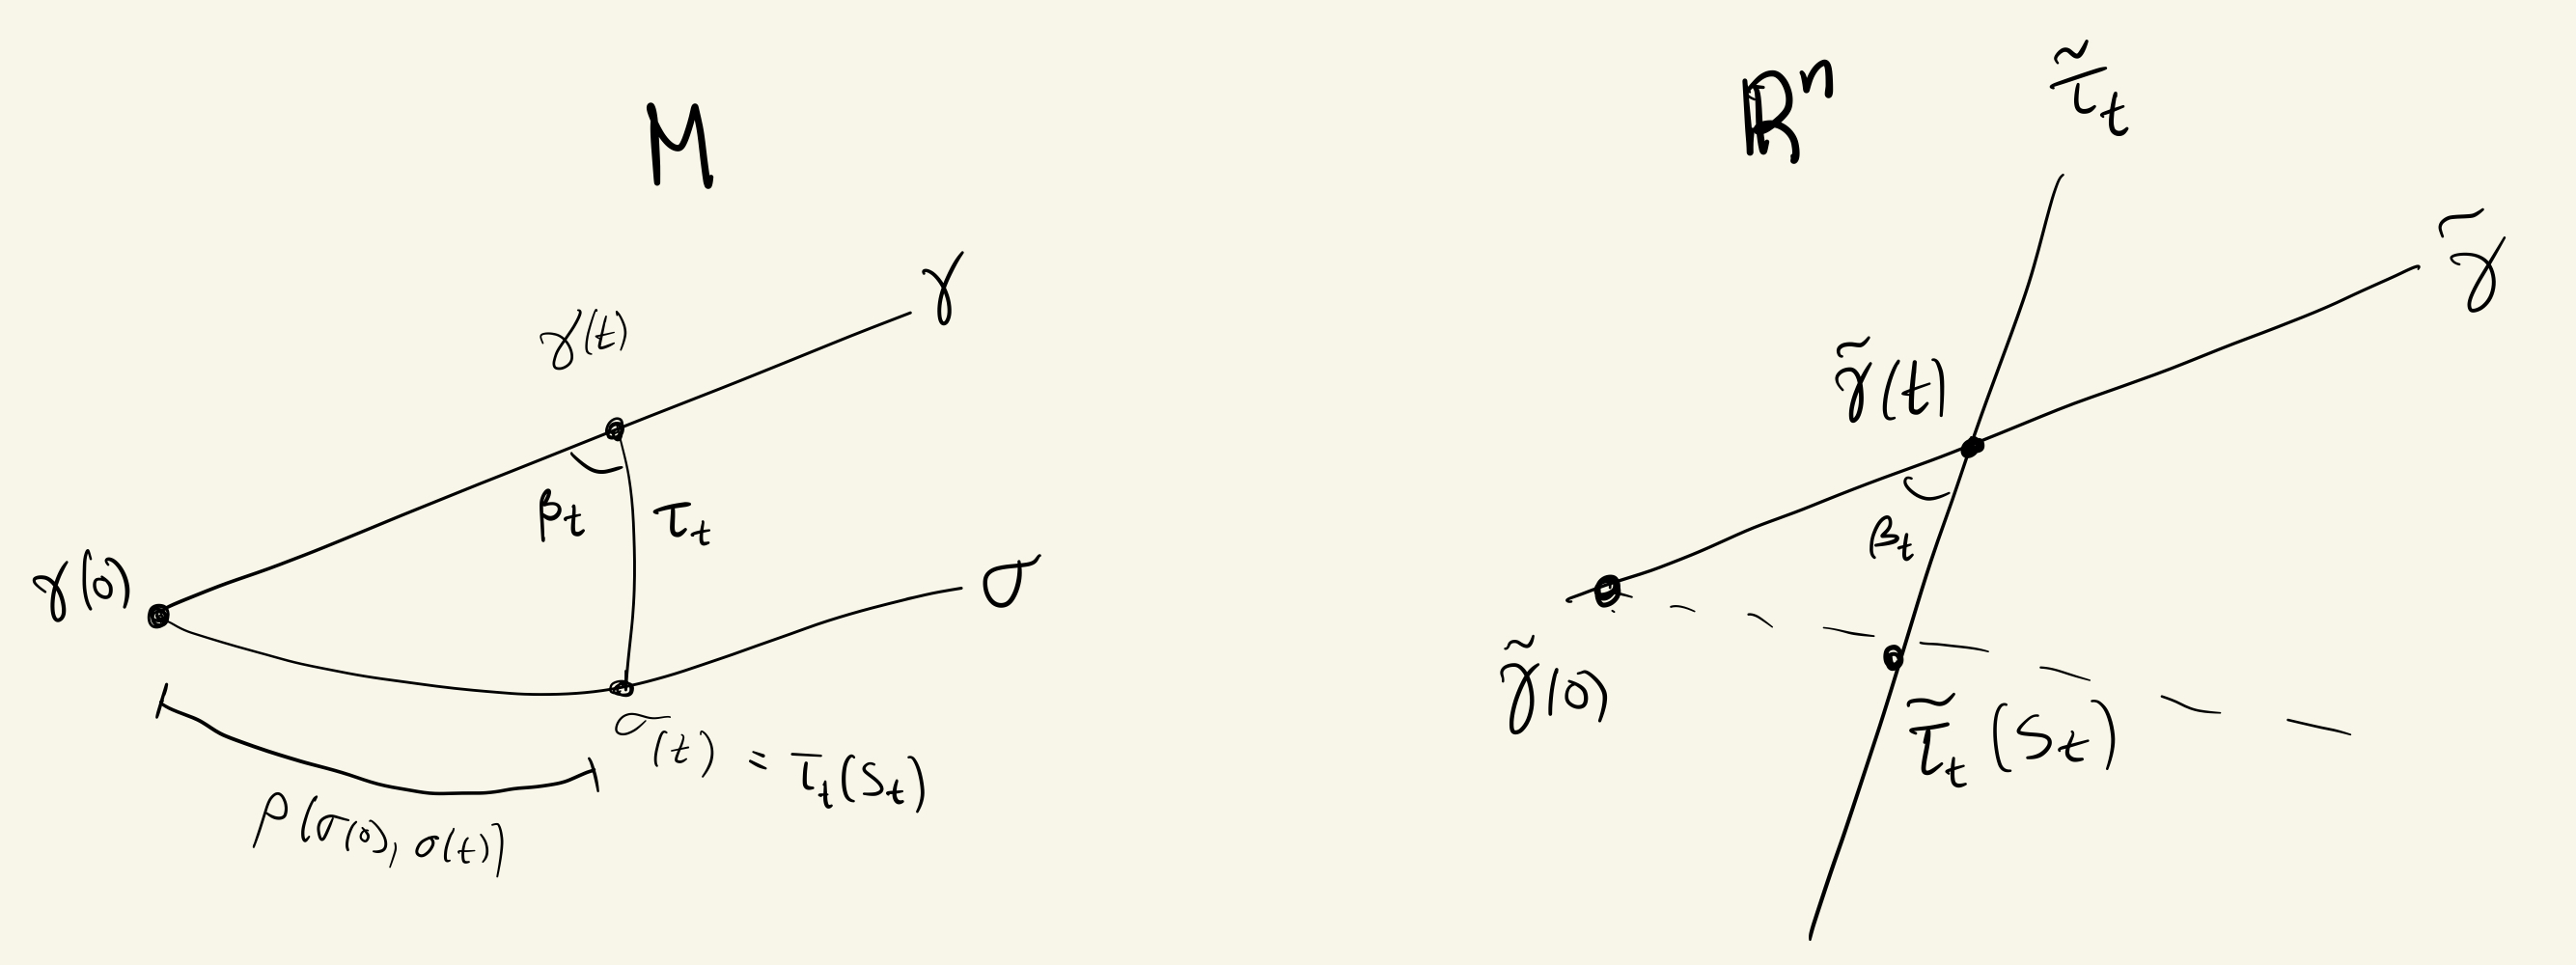
\includegraphics[width=1\textwidth]{figures/toponogov-exercise}
\end{figure}


Como $\tilde{\sigma}$ é uma geodésica no $\mathbb{R}^n$, a distância
 $\rho_{\mathbb{R}^n}(\tilde{\sigma}(0),\tilde{\sigma}(t))$ diverge conforme
 $t\to \infty$, e obtemos o resultado.
\end{proof}



\clearpage
\bibliography{my}
\bibliographystyle{amsalpha}

\end{document}
